%% ----------------------------------------------------------------
%% Thesis.tex
%% ---------------------------------------------------------------- 
%% Final copy must be double sided printing.
\documentclass[twoside]{ecsthesis}      % Use the Thesis Style
\graphicspath{{./figures/}}   % Location of your graphics files
\usepackage{natbib}            % Use Natbib style for the refs.
\usepackage[all]{xy}
\usepackage{float}
\usepackage{mathptmx}
\usepackage{fixltx2e}
\usepackage{listing}
%\usepackage[figuresright]{rotating}
\usepackage{pbox}
\usepackage{multirow,bigdelim}
\usepackage{alltt}
\usepackage{tikz}
\usetikzlibrary{arrows,shapes,automata,backgrounds,petri,shapes.geometric,positioning}
%\removecolourlinks    % Uncomment this command to remove colour from any links
\usepackage{bibentry}
\nobibliography*
\usepackage{color}
\usepackage{soul}
\newcommand{\TODO}[1]{\hl{TODO: #1}}

%\input{Definitions}            % Include your abbreviations
%% ----------------------------------------------------------------
\begin{document}
\frontmatter
\title      {An Investigation into Dialectic and Eristic Argumentation on the Social Web}
\authors    {\texorpdfstring
             {\href{mailto:tb12g09@ecs.soton.ac.uk}{Tom Blount}}
             {Tom Blount}
            }
\department  {Electronics and Computer Science}
\group       {Web and Internet Science}
\addresses  {\groupname\\\deptname\\\univname}
\date       {\today}
\subject    {}
\keywords   {}
\supervisor {Dr David Millard\\Co-Supervisor: Dr Mark Weal}
\examiner   {Dr Nicholas Gibbins}
\maketitle
\begin{abstract}
Argumentation, debate and discussion are key facets of human communication, shaping the way people form, share and promote ideas, hypotheses and solutions to problems. Argumentation can broadly be broken down into collaborative problem solving or truth-seeking (known as dialectic argumentation) and quarrelling without hope for a resolution, either aggressively or for the purpose of recreation, catharsis or entertainment (known as eristic argumentation). Techniques used within argumentation can likewise be classified as primarily fact-based (logical), or emotion/audience-based (rhetorical).

The social web, consisting of the people, tools and communities that form over the world wide web, is a growing way in which individuals, social groups and even corporations share content, ideas and information, as well as hold discussions and debates. As the social web becomes more widely used, the potential for using it as a means to study how people communicate and collaborate on an enormous scale dramatically increases. Current models of argumentation often focus on formal argumentation techniques, in which participants are expected to abide by a stringent set of rules or practices. However, on the social web there is no such code of conduct. Antisocial behaviour, which often stems from argumentation, can have a negative impact on online communities, driving away new users and stifling participation.

Case-studies were carried out on three different areas of the social web to determine the strengths and weaknesses of modelling social, eristic argument on the web when using current models and ontologies. This preliminary work indicates that existing techniques for modelling argumentation are insufficient to capture the structure and dynamic of argumentation taking place on the social web. 
\newpage
Following this, augmentations were made to current modelling ontologies for the purpose of capturing a sub-set of rhetorical tactics. These were then used as part of an investigation re-examining the previous case studies to determine the prevalence of rhetorical tactics in argumentation within areas of the social web as well as investigating correlations that may be drawn between the use of these tactics and the machine-readable characteristic of the post (e.g. length, word-complexity, etc.). It was found that even this small sub-set of rhetorical tactics was regularly employed throughout each case study. Correlations between tactics and post features were also found, although these were not conclusive due to the discrete and binary nature of the features examined.

Based on these observations, future work will focus on extending the argumentation model further to capture additional rhetorical information, due to the importance of these types of interactions. This will be used in an experiment to analyse how different rhetorical and eristic features impacts users of the social web participating in discussion, and how this affects their perceptions of the topic and engagement with the argument. The results of this can then be used to further supplement the model of eristic argumentation on the web.

\end{abstract}
\tableofcontents
\listoffigures
\listoftables

%% -----------------------
%% lstpatch.sty
%% -----------------------
%% lstpatch cannot be distributed with these files. I believe it is only needed if the
%% \lstlistoflistings is used. So this has been turned off by default. Re-add if required:
%% \usepackage{lstpatch}
%% \lstlistoflistings
%% You will need to download lstpatch, possibly from:
%% http://web.mit.edu/texsrc/source/latex/listings/lstpatch.sty
%% -----------------------


\acknowledgements{Thanks to both my supervisors David Millard and Mark Weal for their guidance, advice and support throughout this work. My thanks also go to my partner, for her love and support, and to my friends, who have encouraged and assisted me on my journey. Last, but not least, thanks go to the EPSRC for providing the funding for this work.}
%\listofsymbols{ll}{$w$ & The weight vector}
\mainmatter
%% ----------------------------------------------------------------
%% ----------------------------------------------------------------
%% Introduction.tex
%% ---------------------------------------------------------------- 


\chapter{Introduction}
\label{introduction}

\textit{``A man may be objectively in the right, and nevertheless in the eyes of by-standers, and sometimes in his own, he may come off worst''} -- \citeauthor[The Art of Always Being Right]{Schopenhauer2009}

\section{Problem Space and Motivation}
\label{introduction:problemspace}

Argumentation is fundamental to human communication -- it is how people share new information and new ideas, and propose courses of action that see them carried out \citep{hahn2005circular, Moor2006}. As a result, there is a large amount of research on argumentation from a wide variety of disciplines and topics, including: philosophy, and the nature of fallacies and how they may be critically appraised \citep{tindale2007}; sociology, and the need to differentiate between classical logic and social argumentation due to the need for the capability to reason using only partial knowledge \citep{polos2002reasoning}; law, and the need for measures of certainty and belief when modelling and reasoning over assertions \citep{bertea2004certainty}; and artificial intelligence, and the use of agent-based systems such as dialogue games, as methods for reasoning over argument to determine the victor or the correct course of action \citep{bench2007argumentation, karunatillake2008}.

Argumentation can be (broadly) separated into two categories based on the goals and intended outcome. Firstly, dialectic argument, in which the participants are engaged in rational discourse with the aim of either discovering the particular truth behind a matter, or formulating a solution or resolution for a set of circumstances \citep{kerferd1981}. Secondly, eristic argument, in which there is no clear goal and the participants are not trying to come to a resolution but are quarrelling with the aim of being seen to win, either in the eyes of their opponent or, more often, in the eyes of spectators \citep{kerferd1981, Jorgensen1998}. Arguments can shift between these two forms, or contain ``pockets'' of one form within the other. Orthogonally to this, there are the notions of logic and rhetoric. While often used in modern parlance as a pejorative term, rhetoric is simply the art of discourse, and convincing an audience to one's point of view based on one's knowledge of the topic at hand and, crucially, one's knowledge of the audience themselves (which clearly lends itself to the eristic form) whereas logic deals with reasoning between established facts (which lends itself to the dialectic form).

However, as \citet{Van2004} note, \textit{``perhaps out of fear of metaphysics or of `psychologizing,' present-day logicians tend to concentrate exclusively on formalized arguments that lack any direct relation with how argumentation is conducted in practice.''} Social argumentation, or the way people argue day-to-day, often has a very different structure to formalised models. In these instances, the aim of a proponent is not to prove themselves right through irrefutable logic, but simply to make others believe that they have proved themselves right. 
%\citet{Schopenhauer2009}, in his satirical work \textit{The Art of Always Being Right}, emphasises that \textit{``A man may be objectively in the right, and nevertheless in the eyes of by-standers, and sometimes in his own, he may come off worst''}.

This is particularly relevant when applied to the social web. As a network of social relationships that are created, formed and maintained through the world wide web, the social web (and the social media presented across it) are rife with discussion, debate, and argumentation \citep{rowe2011predicting}. As the web (and in particular the number of people, tools and communities that make up the social web) grows and becomes totally ubiquitous \citep[p.~559]{smith2009social}, the potential for using it to investigate how truly massive communities interact, communicate and argue increases dramatically. However, the social web presents a number of challenges for extracting and analysing arguments, particularly due to the lack of clear indicators of argument structure. This problem is compounded by the type of language used; often highly informal, incorporating slang and irregular punctuation and grammar \citep{Schneider2012}, and by the number of distinct social platforms, each with their own constraints and cultures \citep{hanna2011}.

There are a number of challenges when considering maintaining the social web as an inclusive platform for diverse and vibrant content, especially debate and discussion. There is a tendency for users to interact and associate with others who are similar in terms of traits, (such as race, age, or education) and beliefs (such as religion or politics), known as homophily \citep{sherchan2013} and is compounded by the introduction of ``filter bubbles'', the effect of content providers tailoring search results or default displays towards the preferences of individual users 
\citep{pariser2011}. This can lead to sites becoming ``echo chambers'' in which well-known views and opinions are repeated, little original content is produced and there is virtually no dissent or debate \citep{gilbert2009}. This can be further exacerbated by reputation systems, enforcing which views are acceptable in a given community by rewarding users who agree and punishing those who disagree, or those considered ``outsiders'' of the accepted group or culture. At the opposite end of the spectrum, where there is constant and stimulated debate, there is equal (if not greater) potential for conflict. While critical and reasonable debate, and even (respectful) recreational quarrels, are things to be encouraged, there is a visible tendency to ``shout down'' the opposition, including attempts to silence dissenting opinions through abuse and threats. As a result online communities can become incredibly hostile spaces, culminating in anti-social behaviour, including vulgar abuse and, at the most extreme, threats of sexual violence, and death threats \citep{willard2007, jane2014}. 

However, in this document the case is made that disregarding these interactions from argumentation models is a mistake. Accurately modelling them is the first step towards understanding exactly how argumentation is applied across the social web, and the ways in which creators and consumers of social media engage with argumentation. This information can then be applied towards creating tools and environments that discourage these types of abuse to facilitate more social argumentation.


\section{Hypothesis and Research Questions}
\label{introduction:hypothesis}
One key feature of social argumentation is the notion of the (presence of) an audience \citep{Van2004, jimenez2007}. The audience's perception of the argument is something that is often overlooked in formal models of argument, despite evidence that perception of argument can be altered through multiple means such as cultural associations \citep{suzuki2011}, pre-existing biases \citep{Arceneaux2012} or peripheral information\citep{lee2014}. The ultimate aim of this research is to explore how perception of argumentation specifically on the social web can be altered based on the types of tactics used, and how this can be used to develop more thorough models of argumentation. To achieve this, it is first important to be able to correctly model and represent the arguments that occur socially. In this way, the key features of informal arguments can be identified and categorised. This can then be used to determine exactly which features of argumentation are considered most important by users, and those that they are most likely to engage, reply to, critique, and how these features shape users' overall interpretation of an argument. The work described in this thesis examines how formal models currently map arguments, and applies a combination of these models to an argument (or arguments) on the social web to determine which features are well captured, and those that are not. This has led to the formulation of a hypothesis that the presence of particular rhetorical tactics affects both a user's perception of an argument, and the way in which they engage with it.

This forms the basis of the hypothesis which is examined in the body of this thesis:

\textit{``A model of eristic argumentation on the social web should include both logical and rhetorical tactics, as the inclusion of rhetorical techniques affects the way in which users perceive and engage with the argument''}

This can be resolved into three distinct research questions:
\begin{enumerate}
\item \textit{Is modelling eristic argumentation a valuable direction of work?}
\item \textit{Are current frameworks and tools sufficient to model eristic argumentation on the social web?}
\item \textit{How should rhetorical techniques be included in a model of eristic argumentation on the social web?}
\item \textit{Do rhetorical techniques affect the way in which users perceive and engage with the argument?}
\end{enumerate}

Question one is perhaps the most important question, as it determines the overall value of this work. It is best answered in several different parts; firstly, by literature review, secondly, by an analysis of techniques commonly used in social argumentation, and thirdly by interviewing experts in fields that commonly use, model or support argumentation.

Question two focuses on determining whether it is currently possible to accurately describe argumentation occurring on the social web in terms of pre-existing models. Through a review of existing literature and a short exploratory work in the area, the current state-of-the-art will be examined and their suitability at modelling personal, social, and rhetorical argument will be evaluated.

Question three revolves around the most appropriate means of representing rhetorical tactics. Clearly, providing an exhaustive list of all possible examples of rhetorical tactics would not only be infeasible, but also unlikely to provide any value to modellers or analysts. Therefore, to determine the most effective means of representing these tactics, modellers and analysts should be consulted to determine the most effective method, with an emphasis on the purpose of use.

Question four focuses on the practical implications of this work; that is to say, whether the users of social media perceive arguments using different logical and rhetorical tactics in different ways, and whether this drives them to engage in different manners. This makes it important to define the terms perception and engagement. Perception can be thought of as the way in which users understand the tone, persuasiveness, entertainment value or information content of an argument \citep{sundar2000}. Engagement, conversely, can be thought of as how likely they are to, and in which they respond to or participate in the argument itself. This not limited to replying to a post: users of social media can engage in multiple ways, including replying, sharing or voting \citep{markova2013}.


\section{Report Structure}
Background information on the topic area, both in argumentation and online behaviour, as well as the state of the research field at present, is discussed in Chapter \ref{background}.
A preliminary investigation into the capabilities of current models of social argumentation, and an analysis of the results, is detailed in Chapter \ref{investigation}.
In Chapter \ref{aswo}, these models are developed and adapted to encompass further social and rhetorical information, creating the Argumentation on the Social Web Ontology. This is used to examine the prevalence of a subset of rhetorical tactics in web-based argumentation and their correlation with machine readable features (such as post length, language, etc.). The model is developed further, with additional changes proposed, and review carried out in which experts in several relevant fields (argumentation modelling, linked-and-open data, the social web, and philosophy) were asked to complete a pair of modelling exercises both with and without,the new additions, and then asked a set of semi-structured questions about their experience.
Chapter \ref{case} details further data collection and annotation from sources on the social web, this time in the context of discussions surrounding online news. Again, this data is analysed at a structural level, in terms of both the social structure and annotated techniques. A narrative analysis is then carried out, examining three individual threads as case studies.
In Chapter \ref{perception}, the data gathered in Chapter \ref{case} is used to form the basis of an experiment into the perception of argumentation: how logical and rhetorical techniques affect the perception, and reaction to, arguments on social media.
Finally, Chapter \ref{conclusionsfuture} summarises the overall findings of this body of work, discusses the implications, and makes some suggestions to how this work can be expanded in future.


\section{Contributions}
The work discussed in this thesis has formed the basis of a number of papers:

\begin{itemize}
\item \bibentry{Blount2014}

This paper discusses the preliminary work carried out in Chapter \ref{investigation}, in which an existing model of argumentation is applied to a set of discussions on the social web, an its overall effectiveness evaluated.

\item \bibentry{Blount2015}

This work forms the first part of Chapter \ref{aswo}, in which the Argumentation on the Social Web Ontology is developed, and trialled on a sample of argument data taken from the social web.

\item \bibentry{Blount2015role}

This paper presents a position on one of the issues considered out of scope of the main body of work presented here: namely, do avatars - the visual representation of a person in a virtual world \citep{bailenson2004avatars} - affect they way in which people argue, or the way in which they perceive arguments from others.

\item \bibentry{Blount2016rhetorical}

This work concludes the work begun in \citep{Blount2015}, developing the model further and presenting an expert review of the proposed changes. This forms the final part of Chapter \ref{aswo}.


\end{itemize}
\chapter{Background and Literature Review}
\label{background}

%------------------------------------------------------------------

\section{Rhetoric and Argumentation}
\label{background:rhetoric}
Rhetoric is often used in modern parlance as a pejorative to describe persuasive language that lacks substance, or containing empty or insincere promises; formally, however, it refers to the art of persuasion, whether spoken or written. In particular, it focuses on the act tailoring one's argument to the situation at hand based on knowledge of events and, crucially, knowledge of the audience \citep{Corbett1999}.

\subsection{Modes of Persuasion}
Aristotle, in his treatise on rhetoric, described three ``persuasive modes'' that can be employed in an attempt to sway an audience: through the words that are used (\textit{logos}), through the character of the rhetor or their opponent (\textit{ethos}), and through the emotions of the audience (\textit{pathos}) \citep{Kennedy1991}. These modes may be applied individually, or in conjunction with one another. \textit{Logos} describes an appeal to logic or reason. This is the method by which one might rationalise a position, often backing it up with evidence or statistics. It is important to note that, when enacting \textit{logos}, it is not strictly necessary for the logic to be sound, or the evidence provided to be factual -- it can be warped to fit a particular purpose, or even outright fabricated (however, this will usually also invoke another of the modes described below). The key element is that it appears to be reasonable and thus, appeals to an audience's sense of reason \citep{Kennedy1991, Braet1992}. \textit{Ethos} is an appeal a person's character or sense of ethics and morals. This can be used in an attempt to strengthen the position of the rhetor's argument or to weaken their opponent's position. For example, if a rhetor can state that they are an expert in the field that they are debating then it is likely their audience will lend their argument more credence than if they were a novice. This specific case is known as an argument from authority, or \textit{argumentum ab auctoritate} \citep{Kennedy1991, Braet1992}. Similarly, an argument can be made that attacks an opponents position indirectly, by attacking their credentials rather than refuting their claims (\textit{argumentum ad hominem}). Although such an argument is not logically sound (and constitutes a fallacy), it is still often used in practice and in certain circumstances is a viable (and often effective, if somewhat underhand) means of persuading an audience \citep{walton1987, Budzynska2012}. Finally, \textit{pathos} is an appeal to emotion, whereby an attempt is made to evoke a particular feeling in an audience in the hope that this will influence their opinion on a position. This can be done in both positive and negative terms. For example, flattering an audience, or promising them a boon, can shift them towards accepting a particular course of action. On the other hand, threatening them with the potentially undesirable consequences of their actions can cause them to reconsider even if these consequences are unlikely or, indeed, impossible. A classic example is the appeal to fear (\textit{argumentum ad metum}) \citep{Kennedy1991, Braet1992}.


\subsection{Dialectic and Eristic Argument}
\label{background:rhetoric:dialectic}
The terms dialectic and eristic were coined in Ancient Greece to describe modes of argumentation with different goals and were popularised in Plato's \textit{Republic} \citep{Bloom1991}. A dialectic argument takes the form of two or more parties engaged in rational discourse with the aim of either discovering the particular truth behind a matter, or formulating a solution or resolution for a set of circumstances \citep{kerferd1981}. For example, an academic presenting their findings and rationalising that they are indeed valid, given the rigorous methodology they have used and the weight of evidence this has provided is an example of a dialectic argument. Likewise, a peer reviewer that disagrees with the findings by pointing out a specific flaw in the experimental methodology and explaining how this should be resolved, is another example. The arguments tend to rely heavily on the mode of \textit{logos}. In contrast, an eristic argument is an argument in which there is no clear resolution in the minds of the participants: they are not motivated by solving a problem, or convincing their opponent, but to be victorious \citep{kerferd1981}. There may be different reasons for arguing in this vein, from quarrelling for its own sake as a form of catharsis \citep{Schneider2014}, to being seen to ``win'' the argument in the eyes of spectators \citep{Jorgensen1998}. As a result, these arguments chiefly favour the modes of \textit{ethos} and \textit{pathos}.

\TODO{Polemics} \citep{lemaitre2015}


\subsection{Modelling Argument}
\label{background:rhetoric:modelling}
There are many different models and frameworks used to capture particular aspects of argumentation. These aspects include notions of trust \citep[p.~752]{Wigmore1913}, focus on argument topic or chronology \citep{Klein2010} and the ability to demonstrate support for or refutation of other points in the structure \citep{Dung1995}. Some examples are discussed below, with respect to their technical structure, their influence in the field and their practical applications.


\subsubsection{Toulmin Model}
Toulmin developed his model from the school of philosophy in the 1950s as a means of demonstrating an approach to practical (rather than theoretical) argumentation, by attempting to show the internal structure (and thus, consistency) of an argument \citep{Toulmin1958}. The general form of Toulmin's argument, shown in Figure \ref{figure:toulmin:general}, follows the structure of a \textit{claim}, or conclusion, that is backed up with generally agreed upon facts (the \textit{data}). The \textit{claim} can be \textit{qualified} (``definitely'', ``maybe'', ``probably'', etc.) and any potential \textit{rebuttals} accounted for. Then, key to the Toulmin model, the \textit{claim} and \textit{data} are connected using either an implicit or explicit \textit{warrant}, or justification -- this can then be supported by a particular \textit{backing} \citep[p.~347-350]{Verheij2005}. A specific example can be seen in Figure \ref{figure:toulmin:specific}, which shows an argument reasoning that Alice is a British citizen. Toulmin's model has been a particularly influential piece of work and has had an impact of decades of argumentation research  in fields as far ranging as law, rhetoric and education (\citealp[p.~8-10]{Newman1992}; \citealp[p.~5, 12]{Schneider2013}). However, there has been discussion as to the effectiveness of different aspects of the framework. In its favour, the means of explicitly stating the connecting warrant (and associated backing) can improve cross domain discourse. On the other hand, because models themselves are focused towards internal structure, there is no criteria for modelling overall structure (such as a group of arguments that refutes or support one another's claims). There is also no concept of resolving an argument (for example, on the grounds of logic or value); although this may have been by design, it negates the possibility of evaluating the strength of a given argument (\citealp[p.~349-350]{Newman1992}; \citealp[p.~5, 12]{Verheij2005}). Among other applications, the Toulmin model has been incorporated into the Argument Model Ontology\footnote{http://www.essepuntato.it/2011/02/argumentmodel}, an OWL ontology to allow classification of academic arguments. This is used in conjunction with CiTO, an ontology for factually and rhetorically categorising citations \citep[p.~8]{Peroni2012}.

\begin{figure}[H]
\begin{displaymath}
\xymatrix{
\mbox{\textit{Data}} \ar[rr] && \mbox{So, \textit{(Qualifier) Claim}} \ar[d]\\
& \mbox{Because \textit{Warrant}} \ar[u]& \mbox{Unless \textit{Rebuttal}}\\
& \mbox{Due to \textit{Backing}} \ar[u]&
}\\
\end{displaymath}
\caption{General form of Toulmin's diagram \citep[p.~104]{Toulmin1958}}
\label{figure:toulmin:general}
\end{figure}



\begin{figure}[H]
\begin{displaymath}
\xymatrix{
\mbox{\parbox[t]{0.2\linewidth}{Alice was\\born in Bermuda}} \ar[rr] & & \mbox{\parbox[t]{0.2\linewidth}{So, Alice is (presumably) a British citizen}} \ar[d]  \\
& \mbox{\parbox[t]{0.2\linewidth}{Because a person\\born in Bermuda\\will be a British\\citizen}} \ar[u]& \mbox{\parbox[t]{0.2\linewidth}{Unless both of\\Alice's parents\\were aliens (etc.)}} \\
&&&\\
& \mbox{\parbox[t]{0.2\linewidth}{Due to the\\British Overseas\\Territories Act 2002}} \ar[u]&
}\\
\end{displaymath}
\caption{Example usage of Toulmin's diagram \citep[p.~105]{Toulmin1958}, examining whether Alice is a British citizen}
\label{figure:toulmin:specific}
\end{figure}

\subsubsection{Information-Based Issue Systems}
Information-Based Issue System (IBIS) models are a particular type of dialectic process originally designed to aid in solving so-called ``wicked problems'' \citep{Kunz1970} -- problems of social policy to which there is no clear definition, methodology or even end-goal \citep{Rittel1973}. IBIS models are represented as trees, made up of four different types of node. Firstly, \textit{Issues} represent the problems that need to be solved, or questions that must be answered. Generally, there is one ``root'' \textit{Issue} to be deliberated, but other sub-\textit{Issues} can be created as necessary during the reasoning process. \textit{Ideas} are proposed solutions or answers to these \textit{Issues}, and each \textit{Idea} can then be weighted positively or negatively using \textit{Arguments For} and \textit{Arguments Against}. IBIS models have seen wide usage in the field of design rationale and cognitive ergonomics where the assimilation of collective knowledge is required to solve problems \citep{Conklin1987, Aurisicchio2013}. An example usage of an IBIS model is shown in Figure \ref{figure:ibis}. Because of its dialectic context, the application of IBIS models is ideal when two or more parties are trying to resolve a complex problem, especially if they have differing (or even opposing) stakes. As might be expected, there are many IBIS-like systems used in system-design and knowledge aggregation. Delibatorium\footnote{http://deliberatorium.mit.edu} is a tool, developed by \citet{Klein2010} of MIT, that uses an IBIS approach to solving challenging problems such as \textit{``Is carbon offsetting a good idea?''}. The IBIS approach is invoked to aid the collaboration of large amounts of people separated across space and time by preserving a topic-centric (rather than time-centric) structure. IBIS structures have also been included in an extension to the SIOC ontology devoted to representing argumentation\footnote{http://rdfs.org/sioc/argument}. This ontology uses the IBIS notation of \textit{Issues} and \textit{Ideas} to formalise the process of solving a problem over social media \citep{Lange2008}.

\begin{figure}[H]
\begin{center}
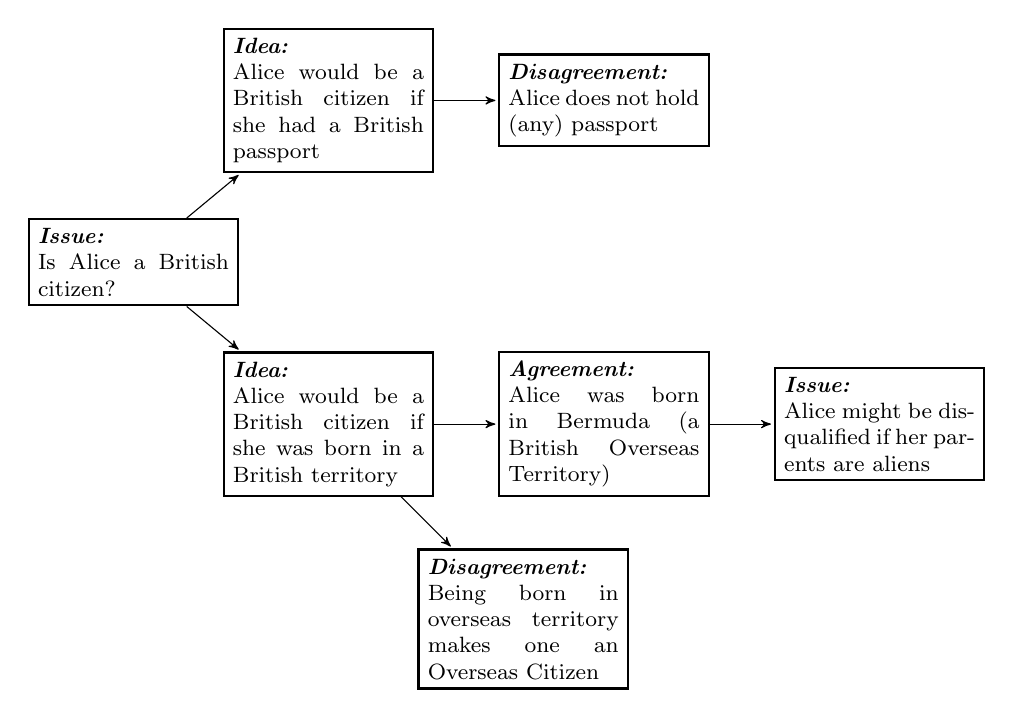
\begin{tikzpicture}[node distance=3.5cm,>=stealth',bend angle=10]

	\tikzstyle{rect}=[
		rectangle,
		thick,
		draw=black,
  		fill=white
  	]
	

	\node [rect, font=\footnotesize] (A) [] {\parbox{0.2\textwidth}{\textbf{\textit{Issue:}}\\Is Alice a British citizen?}};

	\node [rect, font=\footnotesize] (B) [above right=16mm] {\parbox{0.2\textwidth}{\textbf{\textbf{\textit{Idea:}}}\\Alice would be a British citizen if she had a British passport}};
	\node [rect, font=\footnotesize] (C) [below right=16mm] {\parbox{0.2\textwidth}{\textbf{\textit{Idea:}}\\Alice would be a British citizen if she was born in a British territory}};
	

	\node [rect, font=\footnotesize] (E) [right of=B] {\parbox{0.2\textwidth}{\textbf{\textit{Disagreement:}}\\Alice does not hold (any) passport}};
	
	\node [rect, font=\footnotesize] (F) [right of=C] {\parbox{0.2\textwidth}{\textbf{\textit{Agreement:}}\\Alice was born in Bermuda (a British Overseas Territory)}};
	\node [rect, font=\footnotesize] (G) [below right of=C] {\parbox{0.2\textwidth}{\textbf{\textit{Disagreement:}}\\Being born in overseas territory makes one an Overseas Citizen}};
	
	\node [rect, font=\footnotesize] (H) [right of=F] {\parbox{0.2\textwidth}{\textbf{\textit{Issue:}}\\Alice might be disqualified if her parents are aliens}};
	
	\draw[post] (A)--(B)  ;
	\draw[post] (A)--(C)  ;
	
	\draw[post] (B)--(E)  ;
	
	\draw[post] (C)--(F)  ;
	\draw[post] (C)--(G)  ;
	
	\draw[post] (F)--(H)  ;
      
\end{tikzpicture}
\end{center}
\caption{Example usage of an IBIS model, examining whether Alice is a British citizen}
\label{figure:ibis}
\end{figure}


\subsubsection{Wigmore's Chart}
``Wigmore's chart'', conceived in 1913, is a means of recording argumentation originally devised for use in legal trials. The chart models the chain of interactions between competing arguments from both participants and can be used to evaluate the overall conclusion that should be drawn \citep[p.~751]{Wigmore1913}. It takes the form of a directed graph where each node represents a particular fact. The shape of each node relates to the nature of the assertion; squares represent testimony given under oath; a triangle represent an explanation of or support for the node it ``points'' to; an open angle refutes the argument it points to and all other assertions (such as claims, physical evidence or related legal statutes) are represented by circles. These can additionally be marked to denote arguments by the defence or prosecution, but are not discussed here for clarity \citep{Chalamish2011, Chalamish2013}. Symbols relate further information about the nature of these assertions: an infinity symbol ($\infty$) states that a node denotes sensory evidence that may be (re)produced in court; a pilcrow (\P) denotes an assertion that can be taken as fact with no further evidence (such as a precedence case); a lack of a symbol shows that the claim is implied from further reasoning in the graph. In addition, Wigmorean analysis can incorporate the notions of \textit{strong belief} ($\bullet\bullet$), \textit{belief}($\bullet$) \textit{doubt} (?) \textit{disbelief} ($\circ$) and \textit{strong disbelief} ($\circ\circ$) (\citealp[p.~751-756]{Wigmore1913}; \citealp{Goodwin2000}). Little is known about precisely how often this type of analysis is used manually, although it is thought that it is carried out in courthouses around the world \citep{Chalamish2011}. However, efforts are being made to automate the process by parsing the natural language propositions made in court and transforming these into a Wigmore diagram to aid judges, barristers and juries in their deliberations \citep{Chalamish2013}.

\begin{figure}[h!]

\makeatletter
\newif\ifpgfshapebaselesstrianglehasinline
\newif\ifpgfshapebaselesstriangleclose
\pgfkeys{/pgf/.cd,
  baseless triangle apex angle/.style={/pgf/isosceles triangle apex angle=#1},
  baseless triangle inline/.is if=pgfshapebaselesstrianglehasinline,
  baseless triangle has base/.is if=pgfshapebaselesstriangleclose
}

\pgfdeclareshape{baseless triangle}{
  % Copy some stuff from the isosecles triangle
  \inheritsavedanchors[from={isosceles triangle}]
  \inheritanchor[from={isosceles triangle}]{center}
  \inheritanchor[from={isosceles triangle}]{north}
  \inheritanchor[from={isosceles triangle}]{south}
  \inheritanchor[from={isosceles triangle}]{east}
  \inheritanchor[from={isosceles triangle}]{west}
  \inheritanchorborder[from={isosceles triangle}]
  \backgroundpath{%
    % The isoceles triangle defines lots of parameters
    % in the \trianglepoints macro.
        \trianglepoints%
        {%
            \pgftransformshift{\centerpoint}%
            \pgftransformrotate{\rotate}%
            % This bit is a bit of a kludge to ensure the inline
            % is at the top of the figure.
            \pgftransformyscale{cos(\rotate)}%
            \pgfpathmoveto{\lowerleft}%
            \pgfpathlineto{\apex}%
            \pgfpathlineto{\lowerleft\pgf@y=-\pgf@y}%
            % Close the base?
            \ifpgfshapebaselesstriangleclose%
              \pgfpathclose%
            \fi%
            % Draw the inline?
            \ifpgfshapebaselesstrianglehasinline
              \pgfpointdiff{\lowerleft}%
                 {\pgfpointlineattime{0.125}{\lowerleft}{\lowerleft\pgf@y=-\pgf@y}}%
                \pgfgetlastxy{\x}{\y}%
                \pgfmathveclen{\x}{\y}%
                \let\inlineshift=\pgfmathresult%
            % Calculate where the inline hits the sloped line of the triangle.
            \pgfmathparse{\inlineshift/2/sin(\pgfkeysvalueof{/pgf/isosceles triangle apex angle}/2)}%
            \let\inlineendshift=\pgfmathresult
            \pgfpathmoveto{\pgfpointadd{\pgfpoint{0pt}{-\inlineshift}}{\lowerleft}}%
            \pgfpathlineto{\pgfpointlineatdistance{\inlineendshift}{\apex}{\lowerleft}\pgf@y=-\pgf@y}%
        \fi%
    }
    }
}

\begin{center}
\begin{tikzpicture}[node distance=1.6cm,>=stealth',bend angle=45]

	\tikzstyle{circ}=[
		circle,
		thick,
		draw=black,
		fill=white,
		minimum size=6mm
	]

	\tikzstyle{rect}=[
		rectangle,
		thick,
		draw=black,
  		fill=white,
  		minimum size=6mm
  	]
  			  
	\tikzset{
		support/.style={
			regular polygon,
			regular polygon sides=3,
			shape border rotate=90,
			thick,
        	draw=black,
	        fill=white,
        	minimum height=6mm,
        	node distance=0.6cm
    	}
    }
    
    \tikzset{	
		refute/.style={
	    	draw,
	    	thick,
	    	baseless triangle,
 	   		baseless triangle apex angle=60,
 	   		shape border rotate=180,
 	   		baseless triangle inline=false,
 	   		baseless triangle has base=false,
 	   		node distance=0.6cm
  		}
  	}



	\node [circ,tokens=1] (1) [label=above right:$_1$] {};
	
	\node [circ,tokens=2] (2) [right of=1,label=above right:$_2$,label=below right:$\infty$] {};
	\node [support] 	  (2a)[left of=2] {};	
	
	\node [circ,tokens=1] (3) [below left of=1,label=above right:$_3$] {};	
	\node [circ,tokens=2] (4) [below of=3,label=above right:$_4$,label=below right:\footnotesize{\P}] {};

	\node [circ,tokens=1] (5) [below right of=1,label=above right:$_5$] {};
	


	\node [rect,tokens=1] (6) [below of=5,label=above right:$_6$] {};	

	\node [circ] (7)  [right of=6,label=above right:$_7$] {$\circ$};
	\node [refute] (7a)  [left of=7] {};

	\draw[post] (3)-|(1)  ;
	\draw[post] (5)-|(1)  ;
	\draw[post] (4)--(3)  ;
	\draw[post] (6)--(5)  ;
	\draw[post] (2a)--(1)  ;
	\draw[post] (7a)--(6)  ;
	
 
      
\end{tikzpicture}
\end{center}

\begin{tabular}{l l}
\begin{minipage}{0.5\textwidth}
\begin{enumerate}
	\item[$^1$] \footnotesize{Alice is a British citizen}
	\item[$^2$] \footnotesize{Alice has a British passport}
	\item[$^3$] \footnotesize{A person born in a British territory will be a British citizen}
	\item[$^4$] \footnotesize{British Overseas Territories Act 2002}
\end{enumerate}
\end{minipage}

\begin{minipage}{0.5\textwidth}
\begin{enumerate}
	\item[$^5$] \footnotesize{Alice was born in Bermuda}
	\item[$^6$] \footnotesize{Alice's parents testify that she was born in Bermuda}
	\item[$^7$] \footnotesize{Alice's parents' testimony could be biased in her favour}
\end{enumerate}
\end{minipage}
\end{tabular}
\caption{Example Wigmore graph, examining whether Alice is a British citizen}
\label{figure:wigmore}
\end{figure}


\subsubsection{Dung's Framework}
Similar to Wigmore's method, Dung's framework (which uses the format of set theory) focuses on the aspect of arguments attacking, (implicitly) supporting and, ultimately, defeating one another \citep{Dung1995}. Dung defines an \textit{Argument Framework} as a pair such that $AF = \langle AR, attacks \rangle$ where $AR$ is a set of arguments $\left\{a_1, a_2, ..., a_n\right\}$ and $attacks$ is a binary relation such that $attacks \subseteq AR \times AR$. $attacks$ describes which arguments are ``defeated'' by one another: for example, if $a_1$ is the argument ``Alice is not a British citizen'' and $a_2$ is the argument ``Alice has a British passport'' then $(a_2, a_1) \in attacks$. The set of \textit{conflict free} arguments is a maximal set of arguments that do not attack each other. An argument $a_1$ is \textit{acceptable} with regard to a set of arguments $S$ if there is no argument $a_2$ that attacks $a_1$ that is not itself attacked by an argument in $S$. A set of arguments is \textit{admissible} if each argument is considered \textit{acceptable} with respect to the set. The maximal \textit{admissible} set is known as a \textit{preferred extension} \citep{Schneider2013}. 

\TODO{Other extensions}
There have been a number of extensions to this framework.
\citet{Bench-Capon2002} have extended this framework to incorporate the idea of ``value'' or principle to arguments. When circumstances arise such that two possible resolutions to a dispute are equally (logically) valid, different audiences will have differing preferences based on the principles they feel are most important. For example, say that two solutions for combating crime are put forward: reading the general public's private correspondence or an expensive social program of education and rehabilitation. If each has been proven to be equally effective, audiences that value minimisation of cost may favour the former whereas audiences that value individual privacy might choose the latter.
\citet{dunne2016heard} incorporated this to \TODO{FINISH}


\subsubsection{ASPIC}
\TODO{EXPAND THESE}

\subsubsection{ASPIC+}

\subsubsection{IMPACT structured consultation tool}
\TODO{THIS} \citep{wyner2011towards}

\subsubsection{The Argument Interchange Format}
The Argument Interchange Format (AIF) is a framework for representing argumentation as a directed graph \citep{Chesnevar2006}. Created as part of the Argument Web project \citep{Rahwan2007a}, which aims to link the concepts of natural language argumentation with abstract mathematical modelling (including capturing \textit{``linguistically sophisticated manoeuvres''} \citep{Bex2013}), the AIF is primarily a description, with specifications in a number of languages including RDF and SQL.

At its highest level, the AIF can be conceptually divided into an ``upper'' ontology and a ``forms'' ontology. The upper ontology consists of the building blocks of the argument structure, while the forms ontology applies context, for example, by differentiating between logical attacks based on faulty evidence, witness bias, or appeals to authority. The data, claims and conclusions that make up the argument are modelled by Information nodes (I-nodes). There can be no direct relationship between I-nodes. Instead, there must be an intermediary Scheme node (S-nodes). These S-nodes are subdivided into three applications: Rule of Inference Applications (RA-nodes), Conflict Applications (CA-nodes) and Preference Applications (PA-nodes). RA-nodes and CA-nodes simply denote an inference or conflict (logical or otherwise) between one or more pieces of information. PA-nodes, however, denote a preference of one piece of information over another. For example when discussing economics, while it may be difficult to logically prove the superiority of a regulated market over a free market, or vice-versa, the personal beliefs and preferences of proponent and opponent will feature heavily in their reasoning on such issues \citep{Bench-Capon2002}. This structure is displayed in Figure \ref{figure:ontologies:aif}.

\begin{figure}
\begin{center}
\includegraphics[scale=0.42]{./figures/ontologies/aif.png}
\caption{An overview of the AIF Ontology \citep{Chesnevar2006}}
\label{figure:ontologies:aif}
\end{center}
\end{figure}

\subsubsection{AIF+ and Inference Anchoring Theory}

\TODO{Expand details from IAT paper}


In their work on an extension to the AIF, dubbed the AIF+, Reed et al. build on the work of O'Keefe to differentiate between two separate notions of argumentation \citep{Benoit1992, Reed2008}: the first, which they term argument$_1$, is a logically constructed set of claims and evidence used to back these claims (or attack other claims), as in \textit{``Alice put forward her argument''}. The second, termed argument$_2$, refers to a dialogue -- the exchange of ideas and opinions between two or more people, as in \textit{``Alice and Bob were having an argument}. A result of this work was to introduce a new set of nodes. The first, a subset of I-nodes dubbed Locutions (L-nodes), model locutionary acts (or utterances) in an argument$_2$. That is, they record precisely what was said. The second, a subset of S-nodes dubbed Transition Applications (TA-nodes), represent transitions between L-nodes (with associated forms such as a challenge or response). Thirdly Illocutionary Applications (YA-nodes), also a subset of S-nodes, represent the ``illocutionary force'' and serve to link each argument$_1$ to the overall argument$_2$. Figure \ref{figure:graphs:aifplus} shows how this structure can be visualised. Consider the locution \textit{``All men are mortal, and Socrates is a man. Therefore, Socrates is mortal.''} The statement itself is modelled using the L-node on the rightmost side of the diagram. On the leftmost side is the core AIF structure, which show the premises formed as two I-nodes (\textit{``Socrates is a man''} and \textit{``All men are mortal''}), linked to the conclusive I-node (\textit{``Socrates is mortal''}) by way of an RA-node. The L-node is connected to this argument$_1$ by way of the YA-node, shown in the middle.

\begin{figure}
\centering
\includegraphics[scale=0.5]{./figures/graphs/aifplus.png}
\caption{Visualisation of a simple AIF+ graph}
\label{figure:graphs:aifplus}
\end{figure}

\section{Online Communication and Interaction}
\label{background:online}

\subsection{Social Media and the Social Web}
\label{background:online:social}
The social web consists of the people, tools and communities that form over the world wide web, and is a way for individuals to share content, ideas and information. The social web presents a number of challenges for extracting and analysing arguments, particularly due to the lack of clear ``indicators'' of argument or structure. This problem is compounded by the type of language used; often highly informal, incorporating slang and irregular punctuation and grammar \citep{Schneider2012}. As the social web becomes more and more ubiquitous, the potential for using it to investigate how truly massive communities interact, communicate and argue increases dramatically.

Many theoretical models of argumentation are based on the assumption of a dialectic argument, as their purpose is to aid the participants with the process of understanding the information discussed, or to reason over the model and draw conclusions regarding the outcome. However, in social media there is a clear proliferation of eristic argumentation \citep{sood2012automatic}. This makes the role of audience an important feature to consider: when an individual responds to a post on the social web their post is often seen not just by the author of the post they reply to, but by many other users as well. In fact, many posts may be directed at this wider audience to seek approval, voice dissent, or provoke other emotions \citep{berland2010students}. Consider the analogy of a political hustings: neither candidate believe they can change the mind of their opponent, but instead are debating with a view to sway their audience. Schneider et al. note though, that currently it is difficult to model the value of eristic arguments as participants are free to \textit{``sling propositions that they would not commit to under other circumstances''} as a means of catharsis, recreation or entertainment \citep{Schneider2014}.

\citet{Kaplan2010} classify six distinct categories of social media: collaborative projects, blogs, content communities, social networking sites, virtual game worlds and virtual social worlds. Collaborative projects allow many different users to create, maintain and often discuss content. This category includes sites such as the online encyclopaedia \textit{Wikipedia}\footnote{https://en.wikipedia.org/}, which allow users to write and edit articles and \textit{Urban Dictionary}\footnote{http://urbandictionary.com/‎}, a user generated dictionary of slang and internet culture. \citeauthor{Kaplan2010} compare blogs (web-logs) to personal websites, in that they allow users to post information about the subject of their choice -- these posts are often timestamped and presented reverse-chronologically. \textit{Wordpress}\footnote{http://wordpress.com/} and \textit{Blogger}\footnote{http://blogger.com} are two social media sites specialised for this purpose. ``Micro''-blogging sites that pose limits on the amount of content that can be shared in a single post, such as \textit{Twitter}\footnote{http://twitter.com/}, also fall into this category. Content communities revolve around the concept of publishing (and ultimately sharing) different forms of media. These include sites for publishing video (such as \textit{Vimeo}\footnote{http://vimeo.com/}), images (such as \textit{Flickr}\footnote{http://flickr.com/}), audio (such as \textit{SoundCloud}\footnote{http://soundcloud.com/}) and many other different types of media. Social networking sites allow users to create a profile detailing information about themselves (such as home town, or music preferences) and then connect their profiles with the profiles of others on the site. Examples include \textit{Facebook}\footnote{http://facebook.com} and \textit{Google+}\footnote{http://plus.google.com/}. Virtual game worlds (such as \textit{World of Warcraft}\footnote{http://battle.net/wow/}) encompass online games in which a user controls a digital avatar to accomplish certain tasks (such as slaying a virtual dragon, or defeating another player's avatar). Similarly, virtual social worlds (such as \textit{Second Life}\footnote{http://secondlife.com}) encompass virtual spaces in which users have an avatar, but there is no specified aim or end-goal -- the medium exists solely to facilitate social interaction. In this work, less focus is afforded to these latter two areas of the social web due to the the issue that as participants are controlling a virtual avatar, and may be playing a particular ``role'' rather than their real self, this can affect their behaviour and engagement in a discussion \cite{Hooi2013}. There is also the tendency for discussions to centre on the mechanics of the game world itself \citep{alagoz2013}.

\subsection{Anti-Social Behaviour}
\label{background:online:antisocial}
Anti-social behaviour is a growing problem on the social web, and often arises from debates or discussions that get out of hand \citep{suler1998bad, davis2002experience, sood2012automatic}. This behaviour can arise from simple misunderstandings due to the difficulty in conveying tone through text, or as a deliberate act by individuals lashing out at other participants in a discussion. Incidents include
flaming, in which a user simply hurls emotional abuse \citep[p.~13]{Konijn2008}; spamming, in which a user floods the medium with content, often unrelated to the topic in hand, in the hope of drowning out other participants or as a means of advertising a commercial product \citep{krause2008anti}; trolling, in which a user posts seemingly innocuous but deliberately fallacious argument to provoke other members of the group into becoming outraged (although there is debate as to whether this term refers to the bridge-dwelling monster of myths, or the fishing term for dangling a baited line behind a boat) \citep{Herring2002}; 
and much more serious incidents of directed threats and stalking \citep{spitzberg2002cyberstalking, willard2007, jane2014}.

As a result, there is a concerted research effort into the best way to tackle these issues before they cause serious harm to individuals, or the field as a whole. \citet{suler1998bad} discuss a wide variety of approaches (specifically in regard to the virtual social world \textit{The Palace}\footnote{http://thepalace.com}, but these could be applied to other online spaces as well). The simplest solution is to moderate users' interactions and dispense warnings, ``mutes'' (where a user may observe, but not contribute) or, in extreme cases, bans as and when the situation warrants. While effective for dealing with small or close-knit communities, this approach does not scale when considering the social web.

\TODO{Arguments against the troll} \citep{torroni2010}

A different approach is to allow the community a degree of self-moderation. Reputation systems, for example, allow users within a community to assign ``votes'' to a particular account, or post, to show its trustworthiness. This allows new users to make judgements on whether to take a comment seriously, for example, or to purchase something from a particular seller in an online auction \citep{resnick2000reputation, anderson2012discovering}. However, this can also lead to a feedback loop in which communities become self-reinforcing; if users always vote for posts of similar sentiment (or against those that disagree), then gradually these sentiments will become dominant. Over time only users who hold these views will contribute to the site (further reinforcing the disparity) and the community as a whole will stagnate or worse, become distrustful or outright hostile to new members or ``outsiders''.

In another example of direct self-moderation, the popular online game \textit{League of Legends}\footnote{http://leagueoflegends.com} implements a ``tribunal'' system in which players that are reported for poor behaviour in matches (such as verbally abusing team-mates) are judged by their peers. These peers can examine evidence such as chat logs and game scores, then decided whether to ``pardon'' or ``punish'' the offending player \citep{Hodson2013, kou2013regulating}.

A more covert attempt to manipulate users' behaviour can be found in certain implementations of human-computer interaction design. HCI can be leveraged to ``trick'' users into performing (or not performing) an action desirable to the designer. These so-called ``malicious interfaces'' \citep{Conti2010} are often used to trick users into spending time or money that they otherwise would not (for example, advertising banners that suddenly cover page content). In 2008, YouTube temporarily added an ``Audio Preview'' button to its comment system that would read aloud what the user intended to post. This was placed in the previous place of the ``post'' button (which had been moved further to the right), such that a user was likely to unintentionally preview their comment before posting it \citep{Munroe2008}.


\subsection{Modelling the Social Web}
\TODO{Find some more models?}



\subsubsection{Semantically-Interlinked Online Communities}
The Semantically-Interlinked Online Communities project (SIOC) aims to enable the cross-platform, cross-service representation of data from the social web \citep{Breslin2006}. SIOC allows for semantic representations of Sites, which hold Forums, which contain Posts, authored by the owner of a UserAcount. This structure is shown in Figure \ref{figure:sioc}. SIOC is often used in conjunction with the Friend of a Friend (FOAF) ontology, to show how individuals map to their online personas.

\begin{figure}
\begin{center}
\includegraphics[scale=1.75]{./figures/ontologies/sioc.png}
\caption[An overview of the core SIOC ontology]{An overview of the core SIOC ontology\protect\footnotemark}
\label{figure:sioc}
\end{center}
\end{figure}
\footnotetext{http://sioc-project.org/ontology}

While an extension to SIOC, for the purposes of capturing and representing argumentation, does exist \citep{Lange2008}, it is based on the Issue Based Information System (IBIS) principals of modelling an argument as an issue that needs to be solved, with users suggesting ideas, then providing arguments for or arguments against these ideas. While this approach is highly useful when dealing with arguments centred around deliberation, and to a lesser extend criticism or inquiry, they are not as suitable when modelling negotiations or eristic arguments.

\section{Summary}
\TODO{Summarise}
\chapter{Investigating Current Modelling Frameworks}
\label{investigation}
To determine how capable current tools and frameworks are for capturing social argumentation, and the nuances between dialectic and eristic argumentation, a preliminary investigation was conducted. This aimed, firstly, to show how these tools and frameworks can be combined in a way that makes them fit for this particular purpose and, secondly, to determine the key strengths and weaknesses of this combination in relation to modelling social argumentation.


\section{Approach}
The AIF was determined to be the closest fit for purpose ontology for modelling argumentation on the social web, due to the goals of capturing practical, language-based argumentation, with the additional benefit of being readily extensible. Alongside the SIOC, the key elements of these ontologies have been combined to explicitly capture the social component of argumentation on the social web, while also modelling the formalised argument structure. This is achieved by linking the concept of a SIOC Post with that of an AIF Locution, treating a social web thread as a separate dialogue, or argument$_2$ and each post as an atomic unit within the dialogue (containing zero or more individual arguments$_1$). In the majority of cases, a single locution will translate to a single self-contained argument$_1$. However, a single post can contain a number of arguments$_1$ -- each with a number of premises and a single conclusion. In this situation a single L-node will link to multiple YA-nodes, as shown in Figure \ref{figure:graphs:aswo-multiple-ya}. In rare cases (often caused by constraints imposed on the length of a post by the service, such as the 140 character limit on Twitter), a user will spread the premises of a single argument across multiple posts to construct their argument$_1$. Figure \ref{figure:graphs:aswo-single-ya} shows how, in such a situation, multiple L-nodes will link to a single YA-node. If two users post identical statements, they still contribute two distinct locutions. However, they will both be linked to the same I-node(s), and therefore the same argument$_1$. In this situation, multiple YA-nodes may point to the same I-node, such as in Figure \ref{figure:graphs:aswo-repeated-argument}.


\begin{figure}
\centering
\includegraphics[scale=0.5]{./figures/graphs/aswo-multiple-ya.png}
\caption{Visualisation of one post making two distinct arguments$_1$}
\label{figure:graphs:aswo-multiple-ya}
\end{figure}


\begin{figure}
\centering
\includegraphics[scale=0.5]{./figures/graphs/aswo-single-ya.png}
\caption{Visualisation of two posts, used to construct a single argument$_1$}
\label{figure:graphs:aswo-single-ya}
\end{figure}


\begin{figure}
\centering
\includegraphics[scale=0.5]{./figures/graphs/aswo-repeated-argument.png}
\caption{Visualisation of two posts, repeating the same argument$_1$}
\label{figure:graphs:aswo-repeated-argument}
\end{figure}


\section{Methodology}

\subsection{Data Collection}
\label{investigation:methodology:datacollection}
A single topic of argumentation was chosen to be examined for three case studies, each representing a different social media system. To ensure the stimulation of debate, the selected topic needed to be controversial, have a large number of respondents and have been active for a long enough period of time to generate a rich and complete content. The October 2013 United States government shutdown caused by Congress's failure to agree on a budget, and the following condemnation this received from the presidency, was a suitable match for these requirements. 

This topic was then tracked across three of the social media categories identified by \citet{Kaplan2010}: Twitter, a microblogging service that allows users to publish messages of up to one-hundred and forty characters; Facebook, a social network, that allows users to create a network of ``friends'' and share text or images; and YouTube, a content creation site where users can create and upload videos, or playlists of videos.

The source of the posts themselves again needed to be both publicly available and have a large number of followers to ensure a maximally stimulated debate. As an authoritative public figure at the heart of the crisis, content from or relating to Barack Obama's social media profiles was chosen, and three posts that were broadly similar in content were selected for study. The first post, initially posted on 8th October 2013 from the White House's YouTube channel\footnote{https://www.youtube.com/watch?v=7LwoudGfug0}, is a 14m 40s video recording of Obama delivering a statement to press from the West Wing of the White House, condemning the shutdown. The post taken from Obama's official Twitter account\footnote{https://twitter.com/BarackObama/status/390288744235823104} (which is managed by a third party, Organizing for Action), dated 15th October 2013, reads: \textit{``This is unacceptable. Tell Tea Party Republicans to stop holding our economy hostage: http://OFA.BO/qNmA3Y''}. The included hyperlink leads to an Organising for Action page, which encourages users to to voice their displeasure at the shutdown by allowing them to automatically generate and send tweets. The post taken from Obama's official Facebook account\footnote{https://www.facebook.com/photo.php?fbid=10151874920756749} (also managed by Organizing for Action), also dated 15th October 2013, reads: \textit{``Tea Party Republicans in the House of Representatives forced a government shutdown, and now they're threatening an economic shutdown. This has gone on for too long. Tell them to \#EndThisNow: http://OFA.BO/ACC7qB''}.

The discussions surrounding these posts were acquired by collecting comments replying to each initial post, and those replying to subsequent posts in the discussion (taking into account only direct replies, rather than mentions within the text of the post), with the use of the public Twitter, Facebook and Youtube APIs respectively. This data was translated to an RDF triple-store using SIOC to record the data specific to the social media platform, such as which User created which Post and which Thread stores which Posts. This was used in conjunction with the DCTerms ontology, which held supplementary data such as timestamps.

\begin{table}
\centering
\caption{Metrics of total dataset collected from YouTube, Twitter and Facebook}
\label{table:results:totalstats}
\begin{tabular}{| l | c | c | c | c |}
\hline
\textbf{Metric} & \textbf{YouTube} & \textbf{Twitter} & \textbf{Facebook} \\
\hline
Total number of posts 				& 2719 & 137 & 9494 \\
\hline
Total number of users 				& 1255 & 33 & 6224 \\
\hline
Average posts per user 				& 2.17 & 4.15 & 1.53 \\
\hline
Average words per post 				& 26.74& 15.91 & 40.12  \\
\hline
Average characters per post 		& 150.13 & 97.63 & 241.14 \\
\hline
Time between first and last posts 	& 101d 16h 19m 12s & 0d 13h 40m 48s & 90d 19h 55m 12s\\
\hline
Average time between posts			& 53m 52s & 3m 2s & 13m 47s \\
\hline
\end{tabular}
\end{table}


\subsection{Data Sampling and Annotation}
\label{method:annotation}
Because of the volume of the data produced over the course of the tracked event and the time-intensive nature of manually annotating the data, it was necessary to sample the data to a more manageable size before annotation could take place. To prevent information being lost when the dataset was scaled down, it was important to  ensure that the sampled graph maintained properties (such as diameter and average path length) similar to those of the raw data. To maintain these characteristics, ``forest fire'' sampling \citep{leskovec2005graphs, leskovec2006sampling} was used to create a sub-graph that preserved the overall structure of the parent. The algorithm for forest fire sampling is as follows:
\begin{enumerate}
\item Choose a ``forward burning probability'' $p$ -- in this instance a value of 0.7 was chosen based on the recommendation by \citet{leskovec2006sampling} for scaling down a larger graph

\item Choose a random starting node
\label{enum:forest-fire:start}

\item Add this node to the sample graph. Select $x$ nodes at random from all nodes linked to the chosen node, where $x$ is a random number geometrically distributed with mean $\frac{p}{1-p}$. If the selected node has fewer than $x$ linked nodes, select all available nodes, and return to step \ref{enum:forest-fire:start}.
\label{enum:forest-fire:recurse}

\item With each selected node, recursively repeat step \ref{enum:forest-fire:recurse} until the desired sample size has been reached. 
\end{enumerate}

Thirty posts from within the following discussion (i.e. not including the original posts) were selected using this method. This data was then manually annotated with the formal argument$_1$ information. Specifically, from each L-node, both explicit and implicit I-nodes were extracted and related together using the most appropriate S-nodes. %For example, Obama's original Twitter post (an L-node) states: \textit{``This is unacceptable. Tell Tea Party Republicans to stop holding our economy hostage: http://t.co/y8fPF8s3bG''}. From this the following I-nodes can be extracted: \textit{``The Tea Party Republicans are holding the economy hostage''}, \textit{``Holding the economy hostage is an unacceptable tactic''} and \textit{``The Tea Party Republicans should stop holding the economy hostage''}. From this, it is easy to see that the single locution contains two premises and a conclusion (which therefore need to be joined using an RA-node). This argument$_1$ can then be mapped to the specific locution by means of a YA-node.

\begin{table}
\centering
\caption{Metrics of discussions sampled from YouTube, Twitter and Facebook}
\label{table:results:samplestats}
\begin{tabular}{| l | c | c | c | c |}
\hline
\textbf{Metric} & \textbf{YouTube} & \textbf{Twitter} & \textbf{Facebook} & \textbf{All}\\
\hline
Total number of posts & 30 & 30 & 30 & 90\\
\hline
Total number of users & 23 & 12 & 30 & 65\\
\hline
Average posts per user & 1.30 & 2.50 & 1.00 & 1.38\\
\hline
Average words per post & 26.77 & 16.33 & 42.10 & 33.18\\
\hline
Average characters per post & 147.90 & 101.20 & 259.67 & 201.70\\
\hline
Time between first and last posts & 4d 0h 54m 56s & 0d 5h 13m 33s & 3d 12h 13m 18s & n/a\\
\hline
Average time between posts & 3h 20m 31s & 0h 10m 49s & 2h 54m 15s & 0h 17m 10s\\
\hline
\end{tabular}
\end{table}

\section{Results and Analysis}
\label{investigation:results}
An overview of the raw data collected from each platform is shown in Table \ref{table:results:totalstats} and the sampled data in Table \ref{table:results:samplestats}. In total, the discussion generated by the Twitter post has slightly over one-hundred and thirty replies -- in contrast, the  YouTube comments total nearly three thousand posts, and the Facebook discussion has well over nine-thousand. Each platform sees the vast majority of posts contributed soon after the initial post. However, each has a ``long tail'' of responses that gradually decrease in frequency as time goes on. The discussion on Twitter seems particularly ephemeral, with participants only contributing for a short time before moving onto other topics; while the Facebook and YouTube posts appear more ``permanent'', with users finding and contributing to them months later.

\begin{table}
\centering
\caption{Aspects of raw data from social media APIs capable of being modelled using the AIF or SIOC ontologies}
\label{table:method:features}
\begin{tabular}{| l | c | c |}
\hline
\multirow{2}{*}{\textbf{Features present in social media APIs}} & \multicolumn{2}{c|}{\textbf{Represented in:}}\\
\cline{2-3}
 & \textbf{AIF} & \textbf{SIOC} \\
\hline
Locution (explicit content)& $\checkmark$ & $\checkmark$ \\
\hline
Illocution (premises/conclusions) & $\checkmark$ & \\
\hline
Argumentation structure (attacks/support) & $\checkmark$ & \\
\hline
Author  		& $\checkmark$ & $\checkmark$ \\
\hline
Avatar  		&  			   & $\checkmark$ \\
\hline
Replies 		& $\checkmark$ & $\checkmark$ \\
\hline
Creation Date  	& $\checkmark$ & $\checkmark$ \\
\hline
Reputation (e.g. ``Likes'')  &  &  \\
\hline
Location  &  &  \\
\hline
User ``Type'' (i.e. individual/business/etc.)  &  &  \\
\hline
Sentiment (implicit content) &  &  \\
\hline
\end{tabular}
\end{table}

In addition, when collecting this data it became apparent there was information that had no appropriate representation in either ontology, such as reputation systems (for example, the ``Likes'' used by Facebook), the sentiment of the post (for example, sarcasm, humour, abuse) or information about the type of user making the remark (whether they are an individual, a celebrity, a corporation, etc.); these omissions are shown in Table \ref{table:method:features}. These features could have substantial bearing on the perception of the argument$_2$. Consider the example of reputation systems: a retort stating \textit{``You're an idiot''} may be perceived very differently by the audience if it has no up-votes, one up-vote or one hundred thousand up-votes. Alternatively, consider a user making the argument$_1$ that \textit{``I really love using this product''}: whether the statement is made by an individual, or the company selling the product would likely influence the validity and value of the statement.

%\begin{figure}
%\begin{center}
%\includegraphics[scale=0.5]{./figures/lifelines_twitter.png}
%\caption{A subset of thirty Twitter replies, sampled using the forest-fire technique, visualised using Lifelines}
%\label{figure:lifelines-twitter}
%\end{center}
%\end{figure}

%\begin{figure}
%\begin{center}
%\includegraphics[scale=0.45]{./figures/lifelines_facebook.png}
%\caption{A subset of thirty Facebook comments, sampled using the forest-fire technique, visualised using Lifelines}
%\label{figure:lifelines-facebook}
%\end{center}
%\end{figure}

Table \ref{table:results:annotations} shows the statistics collected after annotating the data with premises and conclusions, represented as AIF nodes. Given this data it can be seen that Twitter is the only sample that contains Transition-nodes; that is, replies to other posts within the thread. While this may appear to suggest that the platform is used more fore debate than the others, it is possible this is down to deficiencies in the APIs of the other platforms, which often do not accurately highlight replies. It can also be observed that the debates on Twitter and Facebook have a much higher information content than that of YouTube. The resulting structures are visualised in Figure \ref{figure:speechacts}, which shows a side-by-side comparison of the three different samples.

\begin{table}
\centering
\caption{Summary of AIF nodes found in annotated discussions collected from YouTube, Twitter and Facebook}
\label{table:results:annotations}
\begin{tabular}{| l | c | c | c | c |}
\hline
\textbf{Metric} & \textbf{YouTube} & \textbf{Twitter} & \textbf{Facebook} & \textbf{Total} \\
\hline
L-nodes 			& 30	& 30 	& 30 	& 90\\
\hline
TA-nodes 			& 0		& 20 	& 0 	& 20\\
\hline
YA-nodes 			& 31	& 30	& 41 	& 102\\
\hline
I-nodes 			& 88	& 116	& 110 	& 314\\
\hline
S-nodes 			& 13	& 30    & 26 	& 69\\
\hline
L- to I-node ratio 	& 15:44	& 8:29  & 3:11	& 45:157\\
\hline
\end{tabular}
\end{table}

\begin{figure}
\centering
\begin{minipage}[b]{.30\textwidth}
  \centering
  \includegraphics[scale=0.5]{./figures/speechacts/youtube.png}
\end{minipage}
\hspace{.05\textwidth}
\begin{minipage}[b]{.30\textwidth}
  \centering
  \includegraphics[scale=0.5]{./figures/speechacts/twitter.png}  
\end{minipage}
\begin{minipage}[b]{.30\textwidth}
  \centering
  \includegraphics[scale=0.5]{./figures/speechacts/facebook.png}  
\end{minipage}

\caption{A side-by-side comparison of the emergent structures of discussions taken from YouTube (left), Twitter (centre) and Facebook (right)}
\label{figure:speechacts}
\end{figure}

On the surface, the sample of posts taken from Twitter and Facebook appear to have similar information content. However, upon manual inspection, it can be seen that this average is actually heavily skewed by one particular Facebook post that is thirteen paragraphs long and contains a total of twenty six information nodes. The argument in question is reproduced on a number of different websites, and is likely reused in full as a boilerplate ``cut and paste'' rebuttal by many users when engaging in an argument on that topic.

To highlight the overall information disparity take, for example, the tweet \textit{``@BarackObama Stop expanding government, spying on Americans and driving up the deficit.''}. This is an enthymeme -- the literally derived I-node acts as a conclusion, while the premises (that Obama is expanding government, spying on Americans and driving up the deficit  and that to do so is a bad thing) are left implicit. In turn, contrast with the posts \textit{``first''}, \textit{``wow obama''} and \textit{``lolollll i love this''} which contain very little information, either explicit or implicit. In addition, not all posts with a large amount of literal content have a comparatively large amount of information. For example, posts such as \textit{``Give DIRETIDE Give DIRETIDE Give DIRETIDE...''} (repeated upwards of fifty times in a single post) show a desire to derail the discussion by flooding it with completely irrelevant information (``Diretide'' refers to a cancelled seasonal event in the popular online game \textit{Defence of the Ancients 2}; the cancellation sparking uproar from the fanbase which led to a number of social media platforms being flooded with this message).

In addition, there are other posts that have deeper contextual meaning that would first appear. Consider, for example, ``RedScareBot''\footnote{https://twitter.com/RedScareBot}: this is an automated Twitter account that, using the avatar of Joseph McCarthy (an American politician famous for making claims at the height of the Cold War that their were numerous Soviet agents in the US government), replies to any tweet that includes phrases such as ``communism'' or ``commie'' with quips such as \textit{``Commie Chameleon''}, \textit{``Oh noes, Socialism''} or \textit{``Rise of the USSA''}. While this may seem nonsensical or a non-sequitur without context, \textit{with} context it can be viewed by the audience as a derisive or satirical retort to a knee-jerk insult, despite being posted by a machine.

There are of course limitations on the conclusions that can be drawn from a relatively small dataset when working with proverbial ``big data''. As such, these findings cannot be used to justify broad claims that state that \textit{all} arguments on a particular example of social media are structured in this way. These examples instead serve to demonstrate the important fact that different types of structures \textit{can} evolve, and provide some examples of the argumentative and rhetorical tactics people use when arguing over social media and how the conjunction of the AIF and SIOC projects (as well as any extensions made to these) can be used in attempts to map them.

\newcommand{\scaleProps}{0.7}

\section{Proposals}
\label{investigation:proposals}
These results formed the basis for the work presented in the Workshop on Computational Models of Natural Argument, in which a number of suggestions on how these ontologies could be adapted to model the socio-rhetorical aspects of argumentation were proposed \citep{Blount2014}.

These proposals included suggestions for modelling social web specific features, such as the use of reputation systems. Reputation systems make up a key aspect of non-verbal argumentation on the social web, allowing users to show agreement or disagreement to a position, sometimes anonymously, without the need to articulate their own position. Thought must be given as to how to accurately represent this in a formal model. Figure \ref{figure:cmna:likes2} shows one such approach; namely, modelling each vote as a separate Locution, linking to an I-node that either (logically) supports or attacks the voted-on post. Alternatively, Figure \ref{figure:cmna:likes1} shows an approach which aggregates this information into a single Reputation node. This has the advantage of keeping to social information distinct from the logical graph structure, but the disadvantage of omitting how much each UserAccount contributed to the reputation.


\begin{figure}
\centering
\includegraphics[scale=\scaleProps]{./figures/cmna_proposals/likes2.png}
\caption{Proposal for representing reputation systems by modelling up- and down-votes as individual Locutions}
\label{figure:cmna:likes2}
\end{figure}

\begin{figure}
\centering
\includegraphics[scale=\scaleProps]{./figures/cmna_proposals/likes1.png}
\caption{Proposal for representing reputation systems with the introduction of a Reputation node}
\label{figure:cmna:likes1}
\end{figure}


Another focus of the discussions was that of abusive rhetorical attacks.
Figure \ref{figure:cmna:abuse1} shows the simplest approach, similar to the current way the AIF models the use of \textit{ad hominem} attacks, by linking the attack to the opponent's argument$_1$ with a CA-node. However, this is insufficient for the majority of abusive attacks; while \textit{ad hominem} tactics attack an opponent's argument$_1$ by claiming they are not qualified, or otherwise unfit, to make such an argument$_1$, abuse often does not attack their position at all, but seeks to undermine them emotionally in front of their peers. This mapping can be modelled by linking the content of the locution to the targeted user's account as shown in Figure \ref{figure:cmna:abuse2}. However, a UserAccount can be involved in any number of topics, and be attacked for any number of reasons. Furthermore, a person can choose to present themselves as a dramatically different person (having different credentials, skills, opinions or even race, religion or gender) when they are on the web as opposed to off. They may even choose to represent themselves differently between individual threads and discussions. To this end, another type of node is needed to represent the abstract notion of the ``persona'' a user presents. This is illustrated by Figure \ref{figure:cmna:abuse3}. Introducing the idea of personas allows each UserAccount to present a different view of themselves (that can be supported or attacked accordingly) when engaging in multiple discussions or topics.


\begin{figure}
\centering
\includegraphics[scale=\scaleProps]{./figures/cmna_proposals/abuse1.png}
\caption{Proposal for representing abusive attacks as solely within the argument$_1$ structure}
\label{figure:cmna:abuse1}
\end{figure}

\begin{figure}
\centering
\includegraphics[scale=\scaleProps]{./figures/cmna_proposals/abuse2.png}
\caption{Proposal for representing abusive attacks as connected with the social aspect of the argument$_2$, attacking the author directly}
\label{figure:cmna:abuse2}
\end{figure}

\begin{figure}
\centering
\includegraphics[scale=\scaleProps]{./figures/cmna_proposals/abuse3.png}
\caption{Proposal for representing abusive attacks, extending that shown in Figure \ref{figure:cmna:abuse2} with the addition of Persona nodes}
\label{figure:cmna:abuse3}
\end{figure}

\begin{figure}
\centering
\includegraphics[scale=0.5]{./figures/graphs/aswo-personal-conflict.png}
\caption{Proposal for representing abusive attacks, extending that shown in Figure \ref{figure:cmna:abuse3} with the addition of Personal Conflict node}
\label{figure:cmna:abuse4}
\end{figure}

\section{Summary}
\TODO{Summary}
\TODO{This shows that, currently, it is insufficient to use the AIF (and its extension) to fully model eristic argumentation, even when certain social aspects are  modelled through other ontologies such as SIOC.}
\input{ASWO}
%% ----------------------------------------------------------------
%% Conclusions.tex
%% ---------------------------------------------------------------- 


\chapter{Conclusions and Future Work}
\label{conclusionsfuture}

\section{Findings}
\label{conclusionsfuture:findings}
The work described in this report covers an examination of the capability of current argumentation models, in particular the application of a combination of the AIF and SIOC ontologies to the social web, and the extension of these models to capture social and rhetorical information. Case-studies were carried out on three different areas of the social web to determine the strengths and weaknesses of modelling social, eristic argument on the web. This preliminary work indicated that existing techniques for modelling argumentation were insufficient to capture the structure and dynamic of argumentation taking place on the social web, which led to the publication of a paper in \textit{the 14th workshop on Computational Models of Natural Argument}, detailing these omissions and proposing a set of augmentations to capture additional socio-rhetorical tactics \citep{Blount2014}. These extensions were implemented and trialled as part of an investigation re-examining the previous case-studies to determine the prevalence of rhetorical tactics in argumentation within areas of the social web and look for correlations that can be drawn between the use of these tactics and the machine-readable characteristic of the post such as length or readability. The results of this will published in the upcoming \textit{ACM Conference on Hypertext and Social Media} \citep{Blount2015}. These investigations reveal the following findings.

Firstly, and most importantly, rhetorical tactics are shown to be present throughout the argumentation in the case studies, even when only accounting for a small subset of rhetorical argumentation. Clearly, failure to accurately model these social argumentation strategies is detrimental to the goal of studying how discussions evolve on the social web. Secondly, in the three use cases, rhetorical tactics are most often used by either those contributing the most to the discussion overall, or by those who do not contribute logically at all. Whether this effect is related to a participant's engagement is unknown. However, this raises the possibility that there is a tipping-point in a dialectic logical debate where participants feel the need to expand their use of tactics; alternatively, these users simply interleave both types of tactics throughout their arguments$_2$. Finally, while the features of the argumentation structure above are challenging to detect automatically and expensive to manually annotate, the markers present in the social media sphere are relatively trivial to detect, and some correlations between the two can be observed.

%\subsection{Limitations}
The primary limitation of this work is the necessity to manually annotate all the data. This is time consuming and subjective, but as yet there is no way to circumvent this process and automatically extract premises and conclusions. A further constraint is that only English-language sites are examined. There are, of course, many other social media services that cater to audiences of different languages, such as \textit{Renren}\footnote{http://renren.com/} for China or \textit{VKontakte}\footnote{http://vk.com/} for eastern Europe. However, this separation is mitigated by the fact that different languages (and different cultures) have their own rhetorical structures and argumentation schemes \citep[p.~21]{Van2004}. As a result, attempting to analyse multiple sites with different primary languages concurrently would distort any patterns that might emerge in the argument structure of the users.

\subsection{Hypothesis and Research Questions}
\label{conclusionsfuture:future:hypothesis}
Revisiting the hypothesis initially proposed in Section \ref{introduction:hypothesis}:

\textit{``A model of eristic argumentation on the social web should include both logical and rhetorical tactics, as the inclusion of rhetorical techniques affects the way in which users perceive and engage with the argument''}

This was resolved into three distinct research questions:
\begin{enumerate}
\item \textit{Are current frameworks and tools sufficient to model eristic argumentation on the social web?}
\item \textit{Is modelling eristic argumentation valuable?}
\item \textit{Which rhetorical techniques should be included in a model of eristic argumentation on the social web?}
\item \textit{Do rhetorical techniques affect the way in which users perceive and engage with the argument?}

\end{enumerate}

Based on the proceeding body of work, these questions can now effectively be answered as follows:

\TODO{The first question}

\TODO{The second question}

\TODO{The third question}

\TODO{The final question}


\section{Proposals for Future Work}
\TODO{Further refinement/review of ASWO}
The development of the ASWO has been, and should continue to be, an evolving process. Further refinement and expert review will
This includes returning to the proposals laid out in Section \ref{investigation:proposals}, which discusses other aspects of social argumentation that require additional efforts to model, including the notion of social meta-data such as up-/down-votes.

\TODO{Perception of reputation systems (likes, retweets etc.)}

\TODO{Multi-comment/overall thread perceptions?}


\TODO{Workshop experiment; categorisation/classification of argument tactics; instructed non-experts vs trained non-experts (vs experts)}


Based on the investigations that have been carried out, and the findings described in Section \ref{conclusionsfuture:findings}, there are three particular avenues of future work that could be approached, using this extended model of social argumentation at their core.

Firstly, as is the focus of many researchers in this field, attention can be given to the use of artificial intelligence and argumentation, whether by reasoning over a model of argument in an attempt to determine the most valid argument and subsequent course of action \citep{caminada2007} or by using the model to influence the techniques and strategies of intelligent agents involved in dialogue games \citep{Reed2008}. However, the fact that the eristic features of the model are unlikely to be practical (or appropriate) for the use of reasoning, or governing inter-agent negotiations is likely what has caused them to be currently excluded from the majority of formal models. Disregarding this, the weakness of this approach is that the model cannot, at this stage, be automatically constructed, but must be created through a time and labour intensive process of manual annotation. Therefore, using the model as a basis of reasoning over argumentation in general is ultimately flawed. Any gains that were achieved in this area would be rendered moot by the cost of creating a model for every argumentation to be reasoned over, and rendered impractical on a web-scale.

With this in mind, the second avenue would be to generate this model from the arguments$_2$ themselves, by means of natural language processing \citep{palau2009}, the use of social machines \citep{hendler2010} or some combination thereof. This would go some way towards solving a large outstanding issue in the field \citep[p.~31-32]{Schneider2013}. While working towards a means of automatically generating the model has potential, it is likely that the social and eristic nature of the arguments to be modelled is the very thing that hinders this approach. Web-based culture and language is made up of many disparate groups, and continues to rapidly and constantly evolve, which renders current natural language processing impractical in the short term and ineffective in the long term, without the use of domain-specific normalisation techniques that are expensive or inaccurate \citep{han2011, eisenstein2013}. While the findings in Section \ref{aswo:results} point towards a means of broadly classifying a post as containing different types of logical or rhetorical elements, with reasonable probability, the overall structure may be difficult to model automatically. Clearly, at this stage, human input cannot be wholly eliminated. However, with the use of crowd-sourcing or social machines, the large effort cost of annotating arguments$_2$ could be distributed across participants to a manageable level.

Finally, emphasis could be placed on the social aspect of argument. Because argumentation is a social process conducted by people, it is important to recognise the fact that individuals may perceive the same argument$_2$ in many different ways due to cultural beliefs \citep{suzuki2011}, pre-existing cognitive biases \citep{Arceneaux2012}, as well as features surrounding the content of the argument$_1$ such as avatars \citep{lee2014}. The advantage of this approach is that it uses the existing model as a platform for experimentally evaluating how the use and prevalence of different argumentation tactics affect users' perceptions of an argument$_2$, and the way in which they engage with the thread (and one another) as a result. By using the model as a tool for analysing individual case studies, the requirements for creating and annotating the necessary argumentation structures are greatly constrained, while allowing the findings to be used in further work in the research area. This contribution to the field can then be used to assist further work in a number of other areas, such as another metric for use with adaptive recommendation techniques to match people based on preferred argumentation strategies \citep{guy2010}, or the development of argumentation frameworks that integrate with the social web \citep{torroni2010}.


%\begin{table}
%\centering
%\caption{Example classifications of argumentation posts}
%\label{table:annotations}
%\begin{tabular}{| l | p{10cm} | l}
%%%%%%%%%%%%%%%%%%%%%%%%%%%%% LOGIC %%%%%%%%%%%%%%%%%%%%%%%%%%%%
%\cline{1-2}
%\textbf{Information} & This post contains (purportedly) factual information & \rdelim\}{17}{3mm}[\parbox{3cm}{Logical\\ tactics}]\\
%\cline{1-2}
%(example) & \textit{``Here's a List of 313+ Employers Who Have Cut Hours Because of Obamacare...''} \\
%\cline{1-2}
%\textbf{Logical Support} & This post supports another post or point of view by providing supplementary evidence, attempting to invoke the authority of the author, or another logical tactic \\
%\cline{1-2}
%(example) & \textit{lol, right ? They don't get that if everyone has access to affordable healthcare then everyone pays their fair share} \\
%\cline{1-2}
%\textbf{Logical Attack} & This post attacks another post or point of view by providing contrary evidence, attempting to undermine the authority of the author, or another logical tactic \\
%\cline{1-2}
%(example) & \textit{``No one ``negotiates'' over laws that have already passed''} \textit{``Really? Then why isn't the Volstead Act still the law of the land?''} \\
%\cline{1-2}
%\textbf{Transitionary} & This post attempts to move the argument forwards by asking questions or prompting further debate \\
%\cline{1-2}
%(example) & \textit{``If you know the numbers, then please tell me how many Dems lost their seat the last two rounds?''} \\
%\cline{1-2}
%%%%%%%%%%%%%%%%%%%%%%%%%%%%% RHETORIC %%%%%%%%%%%%%%%%%%%%%%%%%%%% 
%\textbf{Personal Support} & This post expresses support for another user (rather than their argument) & \rdelim\}{15}{3mm}[\parbox{3cm}{Rhetorical\\ tactics}]\\
%\cline{1-2}
%(example) & \textit{``I commend you for admitting that debt \& deficits are important...If only more [people] felt the way you do''} \\
%\cline{1-2}
%\textbf{Personal Attack} & This post attacks, abuses or threatens another user (rather than their argument) \\
%\cline{1-2}
%(example) & \textit{Fuck off cunt} 
%\\
%\cline{1-2}
%\textbf{Calls to action} & Posts that advocate a particular course of action \\
%\cline{1-2}
%(example) & \textit{``Kill them now, impeach them now. The american people dont need masters''} \\
%\cline{1-2}
%\textbf{Meta-argumentation} & Posts that argue about the argument itself -- whether commenting on the rules of the medium or proposing a way participants should argue ``properly''\\
%\cline{1-2}
%(example) & \textit{``Down voting = disagree Upvoting = agree''} \textit{``The rules say explicitly not to do that.....''} \\
%\cline{1-2}
%%%%%%%%%%%%%%%%%%%%%%%%%%%%% OTHER %%%%%%%%%%%%%%%%%%%%%%%%%%%% 
%\textbf{Conversational} & Posts that do not put forward, support or attack a particular view, but make small talk or converse with participants and/or the audience & \rdelim\}{12}{3mm}[Other]\\
%\cline{1-2}
%(example) & \textit{``...I think I am all politically talked out for the night lol, I need to finish some work''} \\
%\cline{1-2}
%\textbf{Off topic} & Posts that do not relate to the topic being discussed\\
%\cline{1-2}
%(example) & \textit{``Ataturk did revolution ! building moderate muslim network is oxymoron which has been destroy secular , democratic, rule of law in Turkey...''} \\
%\cline{1-2}
%\textbf{Other} & The only exclusive category, posts which match none of the above criteria\\
%\cline{1-2}
%(example) & \textit{``[This post has been deleted]''} \\
%\cline{1-2}
%\end{tabular}
%\end{table}
%
%
%%\paragraph{Tasks:}
%%\begin{itemize}
%%\item Recruit annotators
%%\item Conduct annotations
%%\item Check consensus/inter-rater reliability
%%\item Analyse data
%%\end{itemize}
%
%\paragraph{Outcome:} A dataset annotated with a broader sub-set of rhetorical tactics used in nine different argumentative discussions and an analysis of the uses of granular rhetorical tactics across different spheres of the social web.
%
%\paragraph{Estimated Time:} 4 months
%
%
%\subsection{Work Package 2a: Interpretation and Engagement Pilot}
%\paragraph{Description:} To determine an appropriate bounding on the length of experiment and participant overload, a short pilot study will be conducted. This will aim to asses how the number of posts per thread affects the required time for participants to complete the study and the quality and quantity of responses.
%
%%\paragraph{Tasks:}
%%\begin{itemize}
%%\item Recruit participants
%%\item Trial
%%\end{itemize}
%
%\paragraph{Outcome:} Appropriate weightings for participant load during the main experiment described in Work Package 2b
%
%\paragraph{Estimated Time:}2 months
%
%
%\subsection{Work Package 2b: Interpretation and Engagement Study}
%\paragraph{Description:} To determine the effect of rhetorical techniques on the perception of eristic argumentation on the social web, a within-participant experiment will be conducted in which voluntary participants are shown the argumentation threads annotated in Work Package 1b. 
%
%Each participant will be shown three different argumentation threads, each of which originates from a different social media platform. Each thread will be ``pruned'' according to the coarse-grained groups from Work Package 1b so that each users sees one thread containing only rhetorical tactics, one thread containing only logical tactics and one thread containing both rhetorical and logical tactics. Posts that are annotated as containing multiple tactics will be included on a non-exclusive basis (i.e. if a post is marked as containing both logical and rhetorical tactics, it could be displayed in any of the three combinations of tactics). The groups containing rhetorical content will also display social features such as reputation systems. These may need to be normalised across each social biome to prevent participants inferring the likely source platform. The annotations in Work Package 1b cover three different biomes (A, B and C) with three different threads from each (1, 2 and 3), which leads to the proposed potential participant grouping show in Table \ref{table:participant-grouping}.
%
%\begin{table}
%\centering
%\caption{Proposed potential participant groupings}
%\label{table:participant-grouping}
%\begin{tabular}{|c|c|c|c|}
%\hline
%\textbf{Participant Group} & \textbf{$R + O$} & \textbf{$L + O$} & \textbf{$R + L + O$} \\
%\hline
%1 & A1 & B2 & C3\\
%\hline
%2 & C3 & A1 & B2\\
%\hline
%3 & B2 & C3 & A1\\
%\hline
%4 & A2 & B3 & C1\\
%\hline
%5 & C1 & A2 & B3\\
%\hline
%6 & B3 & C1 & A2\\
%\hline
%7 & A3 & B1 & C2\\
%\hline
%8 & C2 & A3 & B1\\
%\hline
%9 & B1 & C2 & A3\\
%\hline
%\end{tabular}
%\end{table}
%
%Datapoints per experimental factor ($D$) can be calculated from the number of threads shown to each participant ($T$), the number of participants ($N$), total tactic combinations ($C$) and the number of different social media biomes used ($B$) using the formula $D = \frac{T \times N}{C \times B}$. Given that the experiment is within-participants, each participant should be shown an equal number of threads and combinations of tactics ($T=C$). This constrains the number (and hence, granularity) of categories that can be examined through this experiment, but ensures that any variance between participants should be controlled for. Therefore, given that three social media platforms will be annotated, for an adequate number of datapoints ($>30$), the number of participants required is $N > 90$.
%
%The presentation of the arguments$_2$ themselves will be in a uniform format, to avoid leading participants to make judgements based on the (perceived) culture of the original platform. Usernames will be semi-anonymised; real names will be removed, as will artefacts revealing the source site (such as the ``@'' prefix used on Twitter), but ``screen names'' (such as \textit{DemsAbroad} or \textit{Tea4gunsSC}) can give an insight to a user's views and motivations \citep[p.~379]{cornetto2006} and while it is conceivable that a participant may have interacted with the user before it is sufficiently unlikely in practice to warrant their inclusion. Participants will need to be regular users of the social web. Given the particular topic of discussion in the dataset, care must be taken to ensure that biases are identified during selection and accounted for during analysis of results. This can also be mitigated through use of a pre-test questionnaire to capture demographic data, topic interest and account for any biases -- due to the topic at hand, this may also require asking participants what they consider their political affiliations.
%
%The majority of questions in the questionnaire will ask participants to rate their agreement with a series of statements on a Likert scale. To determine how participants' perception of the argument$_2$ changes, statements will be based on the work of \citet{sundar2000}, which examines perception of news media by asking participants to rate news stories 
%a series of adjectives including accurate, biased, comprehensive, factual, informative, persuasive, sensationalistic and well-written. The precise adjectives to be used in the survey will need to be resolved to match the platform being examined, but may include statements such as:
%
%\begin{itemize}
%\item \textit{Overall, I found the debate polite}
%\item \textit{Overall, I found the debate informative}
%\item \textit{Overall, I found the debate entertaining}
%\end{itemize}
%
%These can be interleaved with qualitative questions of the form \textit{Please expand on the justification for your choices.}
%
%To determine how participants' engagement may be altered, the Likert statements will take into account the work of \citet{markova2013}, in which they discuss the different types of engagement within social media: consumption, curation, creation and collaboration. These are reflected in the statements chosen:
%
%\begin{itemize}
%\item \textit{I would like to see more posts by these users}
%\item \textit{I would consider responding to this debate by replying with a comment of my own}
%\item \textit{I would consider responding to this debate by voting on these posts}
%\item \textit{I would consider sharing this debate with my friends}
%\end{itemize}
%
%Such questions could be further supplemented with questions of the form \textit{Which user(s) did you find most informative? (Select up to three)}, \textit{Which user(s) did you find least polite? (Select up to three)} or \textit{Which user(s) did you feel had the most powerful argument? (Select up to three)}. This allows, to some degree, the examination of how an individual's posting style can impact the debate, and might also highlight any biases towards certain users and/or points of view. %Additional qualitative questions, such as \textit{What do you feel was the upshot of the debate?} will also be included.
%
%The experiment itself will be run for a period of three months, which should be adequate time to accumulate the necessary participants, with sufficient additional time beforehand to prepare, and afterwards to analyse the results.
%Analysis will compare the responses of participants who have seen the same thread, but different combinations of tactics used, to determine how their viewpoints differ. Comparative evaluation will also show how each user reacts to each tactic-grouping. This will then feedback into the formalised model developed in Work Package 1a, and be written up as a journal article.
%
%%\paragraph{Tasks:}
%%\begin{itemize}
%%\item Plan/form questionnaire
%%\item Create experimental framework
%%\item Recruit participants
%%\item Carry out experiment
%%\item Analyse results
%%\item Write journal paper
%%\end{itemize}
%
%\paragraph{Outcome:} An analysis of the experiment, and a journal paper detailing the process and results.
%
%\paragraph{Estimated Time:} 5.5 months
%
%\subsection{Work Package 3: Write-up of Thesis}
%\paragraph{Description:}
%Having completed these experiments and the analysis of the results, a thesis will be written to describe the findings, determine the effect of rhetorical features on eristic argument and resolve the hypothesis.
%
%%\paragraph{Tasks:}
%%\begin{itemize}
%%\item Write up body of work as thesis
%%\item Have thesis printed and bound
%%\end{itemize}
%
%\paragraph{Outcome:}Printed and bound thesis
%
%\paragraph{Estimated Time:}6 months
%
%
%\subsection{Gantt Chart}
%\begin{sidewaysfigure}
%\centering
%\includegraphics[scale=0.45]{./figures/gantt/gantt.png}
%\caption{Gantt chart detailing the next three Work Packages}
%\label{figure:rhetorictime:Twitter}
%\end{sidewaysfigure}


\section{Conclusions}
Argumentation, like the social web itself, is a diverse construct that is challenging to model but has huge potential if correctly harnessed. Rhetoric and logic are both important aspects of online social argumentation; to accurately model how arguments occur and evolve across social media it is important to take into account all the techniques and tactics that are employed. While it is difficult to determine the value of a contribution, to define all logical contributions (and only logical contributions) as valuable is a naive approach. Being able to accurately record all aspects of argumentation on social media is the first step towards being able to accurately analyse informal argument on an enormous scale. The work presented in this report provides a novel framework for modelling a subset of rhetorical argumentation, ideal for use in modelling social argumentation, and demonstrates some of the structures that may be observed when applied to three case studies. Bringing rhetorical and logical models of argumentation together with the computational modelling of social media argumentation has the potential to be a powerful tool in both our understanding of social media use and social argumentation. This raises the prospects for the development of new tools that could help communities manage argumentation, and counter diverse problems, from echo-chambers and groupthink to trolling and anti-social behaviour.

\backmatter
\bibliographystyle{apalike}
\bibliography{library}

%\mainmatter
%\appendix
%\chapter{Excerpts}
\label{appendix:excerpts}

\section{Twitter}
\label{appendix:excerpts:twitter}
\begin{alltt}\normalfont\textbf{Apologianick}: \emph{@BarackObama I thought a president was supposed to lead...}

\textbf{ItsChris96}: \emph{@BarackObama FOLLOW ME AND ILL REOPEN THE GOVERNMENT}

\textbf{salyvi}: \emph{@thetropico @BarackObama YOU ARE A HORRIBLE PERSON !!  Racist pig!}

\textbf{GSorensen}: \emph{@BarackObama Stop expanding government, spying on Americans and driving up the deficit.}

\textbf{DemsAbroad}: \emph{RT @BarackObama: This is unacceptable. Tell Tea Party Republicans to stop holding our economy hostage: http://t.co/7pD7lA7ZSA}

\textbf{kade6767}: \emph{@Apologianick The president can only so much when idiot republicans refuse to do their jobs properly @BarackObama}

\textbf{Apologianick}: \emph{@kade6767 @BarackObama all presidents must work with Congress. Every budget they've submitted has been turned down.}

\textbf{kade6767}: \emph{@Apologianick Because they have not been clean bills. The president wants a clean bill. That IS doing his job}

\textbf{kade6767}: \emph{@Apologianick Uh, do you not really follow politics or government or even understand it at all? Seriously? Are you learning disabled?}

\textbf{Flandrin78}: \emph{@kade6767 @Apologianick So, because the budget doesn't contain exactly what He wants, Almighty O refuses to fulfill his fiduciary duties?}

\textbf{Apologianick}: \emph{@kade6767 I just expect you to back a claim. Must be hard.}

\textbf{kade6767}: \emph{@Flandrin78 He has no duty to accept unclean bills.}

\textbf{Flandrin78}: \emph{@kade6767 @Apologianick ?..continued... That is completely irresponsible.}

\textbf{kade6767}: \emph{@Apologianick Back a claim? It's not a claim, it's fact. There's the problem with you repubs, too stupid to learn shit on your own}

\textbf{Apologianick}: \emph{@kade6767 when argument fails, ad hominem!}

\textbf{kade6767}: \emph{@Flandrin78 Irresponsible to do his job? Ok, do you not live in the USA or have any clue what a president can and can't do?}

\textbf{kade6767}: \emph{@Apologianick I have no time for fucking morons like you. Follow what the fuck is happening in the country, don't fucking ask for help}

\textbf{kade6767}: \emph{@Apologianick It's your job to fucking pay attention I don't need to do that for you idiot}

\textbf{Tea4gunsSC}: \emph{@BarackObama Mr President u are holding America hostage.}

\textbf{Tea4gunsSC}: \emph{@kade6767 @Apologianick @BarackObama The idiots are those who refuse to talk---u know who u are--if the shoe fits wear it}

\textbf{DelMel_2}: \emph{@Tequilablessed @keshasbestmate @BarackObama very distasteful}

\textbf{theblindsword}: \emph{@Flandrin78 if you believe you're a complete idiot.}

\textbf{Tea4gunsSC}: \emph{@kade6767 How do u think name calling and profanity make u sound or appear to have any intellect}

\textbf{Flandrin78}: \emph{@theblindsword If I said to you that your beliefs make you a complete idiot, what would you say?  Is that any way to constructively argue?}

\textbf{Flandrin78}: \emph{@theblindsword Why don't you come back with your opinion on why you think I am wrong.}

\textbf{kade6767}: \emph{@parisreeves66 That's on the employer as I said. Fear mongering. Blame those employers NOT the ACA}

\textbf{kade6767}: \emph{@parisreeves66 And you'd rather pay higher insurance premiums and pay for the uninsured? That's acceptable to YOU?}

\textbf{kade6767}: \emph{@CMMSJ I mean, don't make comments without understanding what congress does ya know? I know, it's crazy and they always want help}

\textbf{kade6767}: \emph{@CMMSJ because they don't know where to find the info themselves}

\textbf{kade6767}: \emph{@Tea4gunsSC Fuck off cunt}

\textbf{axomamma}: \emph{@Flandrin78 @rakilee @BarackObama You are mistaken. Go look at the numbers.}

\textbf{kade6767}: \emph{@CMMSJ lol, I know I start calling them idiots because at that point it's useless to argue with them, they've won with their experience}

\textbf{kade6767}: \emph{@parisreeves66 I did not say ACA has to end and it was done right. Kinks will be worked out.}

\textbf{Flandrin78}: \emph{@axomamma @rakilee @BarackObama If you know the numbers, then please tell me how many Dems lost their seat the last two rounds?}

\textbf{kade6767}: \emph{@CMMSJ And a big problem is everyone hearing so many untrue facts and they believe everything. Just read the bill. So simple.}

\textbf{BaruckObuma}: \emph{. @BarackObama http://t.co/N6w3jwhO5h}

\textbf{kade6767}: \emph{@CMMSJ lol, right ? They don't get that if everyone has access to affordable healthcare then everyone pays their fair share}

\textbf{stfu_v}: \emph{“@BarackObama: This is unacceptable. Tell Tea Party Republicans to stop holding our economy hostage: http://t.co/6Nd23jxtPu” 

Brainwasher}

\textbf{kade6767}: \emph{@CMMSJ They also don't get if they pay for insurance now, part of out premiums go toward paying for ER visits and the uninsured}

\textbf{stfu_v}: \emph{@CMMSJ @BarackObama OMG stfu}

\textbf{kade6767}: \emph{@CMMSJ Hope you have a great night. I think I am all politically talked out for the night lol, I need to finish some work 😊}

\textbf{clownbabyy}: \emph{@kade6767 @CMMSJ he asked you what was unclean about the bills and you completely dodged the question, don't act like the higher power bud.}

\textbf{Jennster81}: \emph{@Flandrin78 @BarackObama are you drunk Jeremy? I wouldn't want a tea bagger representing me EVER.}

\textbf{Flandrin78}: \emph{@Jennster81 @BarackObama And I didn't want a Lib ever, but society at that time willed it.  Times and majority views are changing though :)}

\textbf{kade6767}: \emph{@clownbabyy I'm not your civics teacher. Try being smart enough to learn on your own. This one is not hard. Unless you're an idiot.}

\textbf{Tequilablessed}: \emph{@tornari117 @CMMSJ @keshasbestmate @BarackObama you don't either!' Stop blaming Him for your mishaps in life,,}

\textbf{kade6767}: \emph{@CMMSJ They don't understand the terminology. Clean bill: only the subject at hand addressed with nothing else attached @clownbabyy}

\textbf{clownbabyy}: \emph{@kade6767 then why didn't you enlighten him on what was wrong with the bills? You follow politics so much surely you could tell him before}

\textbf{clownbabyy}: \emph{@kade6767 resorting to childish acts such as using ad hominems (though this clearly wasn't the case)}

\textbf{clownbabyy}: \emph{@kade6767 I never implied you were my civics teacher and I never asked you to pass knowledge unto me, surely you meant to direct this to him}

\textbf{clownbabyy}: \emph{@CMMSJ you are forgiven, and you did not, in fact you were quite polite in your response.}

\textbf{nonoyawns}: \emph{@kade6767 @Apologianick Is this the part where the Obama apologist starts using insults that demean people with disabilities...? #fail}

\textbf{pbow40}: \emph{@BarackObama follow me off the cliff.}

\textbf{clownbabyy}: \emph{@CMMSJ their views is in question and it turns into a name calling shitstorm, ridiculous.}

\textbf{clownbabyy}: \emph{@CMMSJ well, being constitutionally conservative I believe that when a bill is passed through congress it is a law, the bill was deemed}

\textbf{clownbabyy}: \emph{@CMMSJ I thank you, have a good night!}

\textbf{clownbabyy}: \emph{@CMMSJ thank you soooo much for saying that, that's honestly what I aim for, do keep in mind that I am a dumb teenager though:p}

\textbf{BruessT}: \emph{@BarackObama obamacare is a joke, #united socialist states of america}

\textbf{RedScareBot}: \emph{Socialism lite RT @bruesst: @BarackObama obamacare is a joke, #united socialist states of america}

\textbf{troy0950}: \emph{@kade6767 @Apologianick don't forget the racist part, libtard fallback argument}

\textbf{troy0950}: \emph{@BarackObama don't think so u constitution hating communist}

\textbf{CodyAustin316}: \emph{@BarackObama goodbye freedom, hello socialism. I hope and pray you get impeached.}

\textbf{Dusty_Cole}: \emph{Same logic goes to them, Congress must work w/the Pres just as the Pres must w/them. #Reflexive @Apologianick @kade6767 @BarackObama}

\textbf{RedScareBot}: \emph{Globlist Agenda RT @codyaustin316: @BarackObama goodbye freedom, hello socialism. I hope and pray you get impeached.}

\textbf{kade6767}: \emph{@clownbabyy I don't have a law to follow here as to what I feel like saying, learn to educate yourself not have someone else do it for you}

\textbf{kade6767}: \emph{@nonoyawns That would be republicans that do that you clearly have that backwards}

\textbf{kade6767}: \emph{@StreetForensics One, read what I wrote and two the ACA is only a nightmare if you believe that's what Fox News told you}

\textbf{clownbabyy}: \emph{@kade6767 again I'm not asking you to educate me}

\textbf{kade6767}: \emph{@troy0950 Unless you have something intelligent to add, which of course being a republican you don't, go cry to someone else}

\textbf{kade6767}: \emph{@Dusty_Cole But a president can't make policy or force anything so that is why a president has veto power}

\textbf{kade6767}: \emph{@clownbabyy I'm talking about the other person and I am done with this useless conversation}

\textbf{troy0950}: \emph{@kade6767 not a repub, libtard. You 1st, what was ur word? Oh yea, motherfucker.}

\textbf{kade6767}: \emph{@troy0950 Go get yourself fucking educated you stupid cunt.}

\textbf{kade6767}: \emph{@troy0950 Some of you fucks need a good ass whipping. Please come to Miami, I'll be here til next month idiot}

\textbf{troy0950}: \emph{@kade6767 oh THAT was intelligent! You libtards have such a way with words}

\textbf{troy0950}: \emph{@kade6767 bring it bitch}

\textbf{clownbabyy}: \emph{@kade6767 why}

\textbf{hale_razor}: \emph{@BarackObama Interesting you repeat this "hostage" attack the same day Democrat Filner pleads guilty to false imprisonment.}

\textbf{troy0950}: \emph{@kade6767 blocked me &amp; ran away like the little libtard bitch u are lol}

\textbf{RedScareBot}: \emph{Fools On The Hill RT @georgiapopulist: @tornari117 @BarackObama you wouldn't know socialism if it hit you on the head}

\textbf{kade6767}: \emph{@Gmccormick6 Because they are the ones doing it out of fear not BECAUSE of the ACA, they started doing that the moment it passed}

\textbf{StaceyCripe}: \emph{@BarackObama Dear Dictator Obama, the House is merely exercising their constitutional rights. Try it sometime. http://t.co/LhwbWyjjoj}

\textbf{StaceyCripe}: \emph{@kade6767 @Apologianick @BarackObama They are doing their job. Try reading the Constitution sometime. http://t.co/wd6tGjfmYp}

\textbf{theblindsword}: \emph{@Flandrin78 if they're wrong, then yes.}

\textbf{theblindsword}: \emph{@Flandrin78 the shutdown was orchestrated by the gop. They even changed the rules on how to fix a shutdown on the same day they started it}

\textbf{kade6767}: \emph{@StaceyCripe Congress voted on it. It passed. The SCOTUS upheld it. Obama campaigned on it. GOP doesn't get to complain any further}

\textbf{dj1i}: \emph{@theblindsword @Flandrin78 Tea party are doing what they promised their constituents}

\textbf{theblindsword}: \emph{@dj1i @Flandrin78 them and the republicans have been talking about doing this since 2010.}

\textbf{dj1i}: \emph{@theblindsword @Flandrin78 Supreme Court was supposed to overturn it but didn't}

\textbf{theblindsword}: \emph{@dj1i @Flandrin78 because republicans changed the rules on who can turn over a shutdown.}

\end{alltt}

%\section{Facebook}
%\label{appendix:excerpts:facebook}
%\begin{alltt}
\normalfont
\textbf{100002475047373}: \emph{I want eeuu to enter default}

\textbf{100002541057840}: \emph{(Y)}

\textbf{100000099448491}: \emph{Need to stop this now and start America fresh}

\textbf{100000604568244}: \emph{They're big spoiled brats!}

\textbf{1448332271}: \emph{End it!}

\textbf{100000439344389}: \emph{In NJ vote for Cory Booker tomorrow.  The last thing we need is another sellfish republican}

\textbf{100001615644558}: \emph{Why aren't they all arrested and tried for treason}

\textbf{1815296962}: \emph{Impeach OBAMA and it will END!!!}

\textbf{1203909209}: \emph{Dem & rep all crooks & all need to go! End corporate america replace all politicians with school teachers}

\textbf{1344557634}: \emph{Without money maybe you can finally stop your useless and inhuman wars and start to care at your people mr President}

\textbf{1446489575}: \emph{There's nothing more annoying than a broke republican!!!}

\textbf{514223776}: \emph{Please Mr Obama is there anyway that you can force them to stop this shutdown. ..it's gone long enough. ..and we the poor will pay the price}

\textbf{632262577}: \emph{http://www.youtube.com/watch?v=cpoauPwY0rU&feature=player_embedded}

\textbf{1393291060}: \emph{They are kidding right....they are kidding me right.....ooohhhh it's about to get on and poppin....bring the economy shutdown.....see how well that goes w/u.....remember if the little ppl can't work...big ppl like Uhm the republicans won't get paid either.....we could do this all day.....when revolutionary starts evolutionary thats when things goin to get crazy.....then we destroy each other and that will b THE END......smh.....sad ending}

\textbf{1542871399}: \emph{Just because your side lost the election and you didn't get your way doesn't mean you teabaggers have to go all seditionist on us. America !  love it, or leave it.  Dont say you are a " patriot" if you can't even abide by the basic laws of this great country. The deficit is down more than 40%;  GDP is on the  upswing and the economy has improved. Funny all you " patriots"  were so quiet when Bush was driving us into the ditch.}

\textbf{1341223950}: \emph{Stay firm Mr. President !   God Bless !!!}

\textbf{802655642}: \emph{I just wish we would pass a budget that showed us removing our debt}

\textbf{100001214313621}: \emph{The Tea Party wants to default on our debt to prove to us all that they are in control ...they are ruining our country and everything we stand for}

\textbf{100000182147310}: \emph{Ill never vote again}

\textbf{668175153}: \emph{Private owners taking public resources for themselves are a political interest too. You don't have to have a political party name beside your name to have a political agenda.}

\textbf{100000816166660}: \emph{Dear mr obama,

                           your oppsition party want to prove u a week president.and people don't want a week leader.so my idol leader plese think some new.fro whole country.}

\textbf{1585221143}: \emph{Again there is no Bankruptcy court in the sky to bail us out is there and if we look how much we owe we are worth not much are we? So we are not the richest country in the world any more and that is all you guys fault. Really why don't all our reps let the people know how much they make> av &196,000.00 severance pay to make the fortune 500 envious, and some even if they die the wives get a pay check!!!! They can only make an extra $35,000.00 a year after pay but if they have a business or in the name of spouse or trust fund they can still get dividends, they can sell books and make as many speeches with ample pay. The many speeches and speaking engagements all for a price, and campaigning is imperative in the schedule and  than last but not least we the people. Maybe when people cause mayhem it feels better if the rest world is in mayhem with us have a free for all than people won't complain?}

\textbf{100006744933199}: \emph{Is the shutdown of america is due to nearness with iran & israel is anger for that & the whole economy of america is in hand of israel.so obama excuse with iran & give the happy to his step son istael.}

\textbf{100005327682497}: \emph{are billionaires get hurt every time this unproductive, congress has made the fight and hurt all americans to the turn of 3 trillion dollars all because they do not like a black president , we voted the numbers are in for over 8 years , and over runs and high cost to we the people all because of this pot smoking republican congre  !!!!}

\textbf{1545944548}: \emph{the house wants a bill where  prez and others r not exempt from obamacare, and  Obama says no.  So who r u going to blame for this}

\textbf{100000280675860}: \emph{Tea party republicans in Congress are a living, breathing, walking, talking argument for birth control.}

\textbf{1064820047}: \emph{Republicans....why y'all so selfish?!}

\textbf{100003504710492}: \emph{YES, stop the Madness!!!!}

\textbf{1636115397}: \emph{Those who vote democrap in next election will be signing a death warrant for this country. How much more can Americans take before it all crumbles? We need to get back to our morals and compassion for all Americans, we cannot do that with the current resident in the White House. Read this and maybe...just maybe you will begin to see the light.   http://www.foxnews.com/opinion/2013/10/10/mr-obama-presidency-is-no-place-for-amateurs/}

\textbf{758192074}: \emph{I told you so!}

\textbf{1377522722}: \emph{All of them should be fired}

\textbf{100000077125493}: \emph{GET RID OF ALL OF THESE " TEA PARTY BASTAEDS" Out of Congress........Start with them 2 (POS's......Boehnor and Cantor)}

\textbf{1354163800}: \emph{Isn't it [congres] already ended? Isn't that the point?}

\textbf{561778718}: \emph{More like kinda garden tea party carry on}

\textbf{1417541051}: \emph{they are the reason for everything that has gone wrong in american history. look it up. EVERY LAST BLUNDER BY A REPUBLICAN'T}

\textbf{224783034340255}: \emph{Ataturk did revolution ! building moderate muslim network is oxymoron which has been destroy secular , democratic, rule of law in Turkey. now our state is decayed , PM Erdoğan controls all state institutions. Mr. Obama , your  the great middle east project has turned into radical islamist in the middle east, especially in Syria , in Turkey. you don't have right to change regime of sovereignty states that is enthnocentricism led to fascism in the middle east. let's allow sovereignty nations act by themselves. You don't have right to stop Turkish enlightenment ! Atatürk established Turkish Republic, not George Washington. Turkey is ally with the NATO. but it doesn't mean Turkey is 52  city of the USA. we are independent nation that is Turkish nation. don't divide us ethnic, religious line , stop imperialism. Actually neo-liberalism is not only destroy foreign countries which the USA is selling it, it destroyed the USA economy. this fact was  indicated  few centuries ago by Immanuel Kant who said if state is getting bigger and bigger, it begins to lose, you cannot control whole states and nations. because people like freedom and independent , hate imperialism. think about  the US prestige around the world, nothing. so you don't have right to destroy American's honor, too. many American friends told me that we don't have power to stop the USA foreign policy. there is two political party, we just vote for it. therefore listen to ordinary peaceful people instead of brutal oil and weapons companies. thanks http://www.youtube.com/watch?v=ES-gd8CdUps}

\textbf{1268547410}: \emph{Can we DE-PORT them to Iran}

\textbf{1202881117}: \emph{END THIS NOW!!!!!!!!!!!!!!!!!!!!!!!!!!!!!!!!!!!!!!!!!!!!!!}

\textbf{686665622}: \emph{https://www.facebook.com/photo.php?fbid=578369338867398&set=a.489104871127179.97989.475633619140971&type=1&relevant_count=1}

\textbf{100003814790567}: \emph{The best example of how utterly clueless the Republican rank and file are and what a shameless bunch of liars the Republican leadership is, is the fact that George Bush ran as a "political outsider" even though his father had been President, vice president and head of the CIA, his grandfather was a senator and career politician and his brother was governor of Florida.

How much more of an insider can anyone be?

At this point the Republican party simply lies out of habit. It's always worked for them in the past, why should they stop now?}

\textbf{100000203984762}: \emph{Truth, you want it? Republican anarchists have taken the rest of the republicans hostage too, they changed the house rules so that the majority of the republicans do not override the few republican anarchist who planned the government shutdown. the republican anarchists as of Oct 1,2013 changed house rule 22 clause 4 so that no other republican could reopen government. House rule 368 section 2 only allows the leader and his designee to reopen government, so in short words only the republican anarchist house leader can reopen government. Hmmmmmm, so they blame their brother for spilling the milk, but it is republican anarchist who are exercising tyranny.}

\textbf{538134987}: \emph{Dear....you all are like sheep to the slaughter and you don't even realize it.  Obama will literally strip you of everything you know so he can become dictator of what he thinks is going to be another 3rd world country.  It doesnt matter if you are democrat republican tea party liberalist......Obama dont care...he just wants you life.}

\textbf{1214268832}: \emph{Fitch Ratings has placed the United States on Rating Watch Negative on the high risk that US authorities will not raise the debt ceiling in a timely manner before the Treasury exhausts extraordinary measures on 17 Oct.}

\textbf{100001065167437}: \emph{Kill them now, impeach them now. The american people dont need masters}

\textbf{792805014}: \emph{this totally sucks!}

\textbf{100004617033907}: \emph{GOP brought down a country of 240 years of history in only 16 years, they spent 12.000.000.000.000 $ on those 16 years which is 75% of our current debt, and they have the stone face to blame the black president. You have to be very ignorant to actually believe them}

\textbf{1220771846}: \emph{End Obama NOW!}

\textbf{100003963291599}: \emph{Amen}

\textbf{1068817769}: \emph{http://dailycaller.com/2013/09/30/company-with-1-2-billion-obamacare-contract-under-investigation-for-serious-fraud/2/}

\textbf{1224048062}: \emph{Here’s a List of 313+ Employers Who Have Cut Hours Because of Obamacare 

Houston County
Biola University
Bealls Inc. (Department Stores)
SeaWorld Entertainment
Palmer Place Restaurant
Salina Family YMCA
Middletown Township Public Schools
Sam Houston State University
Auburn Hills
Friendship Community (group home for adults with disabilities)
Meridian Public Schools
Michael Monti’s La Casa Vieja steakhouse
Hollywood Casino
Arizona State University
Mainesubway (Subway franchisee)
Finger Lakes Community College
Tsunami Surf Shops
Southern Illinois University
Vincennes
Mexican American Opportunity Foundation
Georgia Military College
Vcm Inc. (Subway franchisee)
Ball State University
Tom’s River
Forsyth Technical Community College
Wilkes Community College
Consolidated Restaurant Operations Inc
Dave & Buster’s
Philadelphia University
K-VA-T Food Stores
Three Rivers College
Bergen Community College
University of Alabama
Brevard County
Buca di Beppo restaurant chain
Hillsborough Community College
St. Petersburg College
Cherokee County School Board
Hancock County
Morgan County
Central Michigan University
NEMF trucking company
Henderson
White Castle
Shari’s restaurants
Carnegie Museum
Oneida Special School District
Scott County School System
Stewart County School System
Jim’s Restaurants
Christoper Savvides restaurant & catering co.
Minocqua-Hazelhurst-Lake Tomahawk School District
Trig’s Supermarkets
University of North Alabama
Fatburger
Lee County
Delta County
Bee County
Boundary County
Rutherford County
Lawrence County
Kenowa Hills Public Schools
City of Burlington Public Schools
Lion & Rose British Restaurant and Pub
MTC Inc. restaurant management
Millard School District
Pulaski Technical College
San Diego Community College District
Drury University
Cumberland University
Area Agency on Aging of Western Arkansas, Inc.
Wal-Mart Stores Inc.
CKE Restaurants Inc.
Kern County
Rancho Cucamonga
San Gabriel
Palm Beach State College
Santa Fe College
Tallahassee Community College
Parkland College
Clay County
DeKalb County
Eastbrook Community Schools
Floyd County
Highland
Indiana University
Ivy Tech Community College
Kosciusko County
Lakeview Christian School
Madison Consolidated Schools
Madison-Grant United School Corp.
Marshall County
Mississinewa Community Schools
Perry Central School Corp.
Shelbyville Central School System
Speedway Schools
Starke County
Wolfe’s Auto Auction
Spencer Community School District
Lexington Board of Education
Howard Community College
Russ’ Restaurant
Maritz Research
Blair Community Schools
Plattsmouth Board of Education
Little Falls Board of Education
Lake Township
Lebanon City
Mason
Scrambler Marie’s Restaurants
Westlake
East Penn School District
Southern Lehigh School District
Tredyffrin-Easttown School District
Kelly Professional Cleaning Services
Spartanburg Community College
Matagorda County
Wilson County
Murray School District
Nebo School District
Henrico Country School District
Lynchburg
Clyde’s Restaurant Group
Eminence Community Schools
Faribault
Martin County
Baldwin Public Library
Hayfield Community Schools
Rappahannock Area Community Services Board
Benton Community Schools
Pompton Lakes Board of Education
Sparta Area Schools
Brandywine Heights Area School District
Southern Utah Unversity
Arkansas State University
Texas Christian University
Maricopa Community Colleges
University of Arizona in Tucson
Long Beach
Circle K Southeast
College of DuPage
McHenry County College
Eastern Hancock School Board
Fayette County School Corp.
Fort Wayne Community Schools
Gibson County
Greencastle Community Schools
Hancock Madison Shelby Educational Services
Tipton County
Vigo County School Corp.
White River Valley School District
Zionsville Community Schools
Indianola Community School District
Tama County
Kansas Turnpike Authority
Republic Foods (Burger King franchise operator)
Birmingham
Dearborn
Iosco County
Tuscola County
Douglas County West Community Schools
Papillion-La Vista school district
Westside Community Schools
Carlie C’s
Sinclair Community College
Tipp City
Ephrata Area School District
Dallas County Community College District
Plano
Alpine School District
Deseret Industries (work training for war refugees)
Wise County School Board
Mount Horeb Area School District
Tehama County
Crawford County
Vanderburgh County
Campbell County Social Services Dept.
Dickenson County Public Schools
Grayson County
Strasburg
Wythe County
North Putnam Community Schools
Northwestern School Corp.
Taylor Community Schools
Hanover Township
Middletown Township
Cedar City
Dallas School District
New Mexico State University
General McLane School District
Blue Ridge Community And Technical College
Fountain Fire Dept.
North of the River Recreation and Park District
Charco Broiler
Durango
Mountain Del (Del Taco franchisee)
Daytona State College
Moraine Valley Community College
Bartholomew County
Delaware County
Northwestern Consolidated School District
Richland-Bean Blossom Community School Corp.
Clear Lake School Board
Ocean City
Kalamazoo Valley Community College
St. Clair Community College
Moberly Area Community College
Ralston School District
Springfield Platteview Community Schools
Community College System of New Hampshire
Franklin Township Board of Education
Waldbaum’s Supermarket
Cuyahoga Community College
University of Akron
Upper Arlington City School District
Firstaff Nursing Services Inc.
Lancaster County School District
Penn Manor School District
Susquenita School District
Regal Entertainment Group
Brigham Young University
Chesterfield Public Schools
Chippewa County
Tazewell County
Eastern Greene Schools
Portage
Vassar Public Schools
Richmond Public Schools
Spotsylvania County
Joe Bologna’s Italian Pizzeria & Restaurant
Clinton-Glen Gardner School District
Elmhurst College
Columbus State Community College
AAA Parking
Boone Community School District
Joliet Junior College
Van Buren Township
Mankato
Hudson Valley Community College
Five Guys Burgers and Fries franchise
Akron
Baldwin-Wallace University
Kent State University
Lakeland Community College
Youngstown City Schools
Lori’s Angels home care
Granite School District
Chesterfield County
Louisa County
Bowling Green State University
Medina City Schools
Carnegie Library of Pittsburgh
Fairview Park
Shawnee State University
Miami Dade College
Putnam County
Cutchall Management restaurant company
Mount Ephraim Board of Education
CY Farms
Brunswick
Medina
Wytheville Town Council
Christopher Newport University
College of William & Mary
Norfolk State University
Virginia government (all other departments)
Virginia Commonwealth University
Virginia Community College System
Virginia Dept. of Alcoholic Beverage Control
Virginia Dept. of Conservation and Recreation
Virginia Employment Commission
Washington County
Wytheville
Land’s End
Dept. of Behavioral Health and Developmental Services
Dept. of Motor Vehicles
George Mason University
James Madison University
Longwood University
Old Dominion University
Radford University
University of Mary Washington
Lomira School District
Lancaster County
Utah Valley University
Columbus
Illinois Valley Community College
Milford Township
New Baltimore
Omega Foods Inc. (Wendy’s franchisee)
Tallmadge
Treadwell Enterprises (Taco Bell franchise operator)
Lake County
Boca Raton
Rock Valley College
Royal Farms convenience stores
Fairlawn
Chesapeake College
Sugarcreek Township
RREMC Restaurants (Denny’s franchisee)
Cedar Falls
Kga Group (Subway franchisee)
Kean University
Stark State College
Youngstown State University
Community College of Allegheny County
Pillar Hotels & Resorts
PMTD Restaurants LLC (a franchisee of KFC)
Jimmy John’s Gourmet Sandwiches
Plainfield Park District
Bowlmor Lanes
West Perry School District
Lafayette School Corp.

This isn’t just a list. This represents millions of lives damaged by an out of control president, congress, and Supreme Court. It’s time to fight back.}

\textbf{100000485887885}: \emph{I agree with Kate}

\textbf{100000140313752}: \emph{Amen!  This president is bankrupting our country, he is disrespectful to our troops and could care less about it!  Wise up people! He has it made for the rest of his life while we pay off the debts!}

\textbf{100005782921113}: \emph{I am speaking to you before it happens. I AM YOUR REAL PRESIDENT. I AM THE REASON WHY THE GOVERNMENT SHUTS DOWN LIKE MY SYSTEM BY THE BAK. I AM FROM SHENOUDA COUNTRY EGYPT, AND I LIVE IN CANADA. I ORDERED THE MAKING OF THE AMERICAN NEW BAK AS AMERICANS BECAME BAKS. I AM THE ONE. I AM THE MAN. I MADE YOU AND YOU ARE MINE. LEND ME A HELPING HAND SO THAT WE CAN MEET AND SPEAK, AND SO THAT I CAN LEAD.I AM TALKING TO YOU 2 DAYS FROM THE GLOBAL DISASTER AND AN AMERICAN RECESSION. ....}

\textbf{100001918863791}: \emph{Damn tea party........}

\textbf{100003145330402}: \emph{All you tea party sheep listen up. Educate yourself with facts not rhetoric. Go to your church & pray for your own racist anti black and anti Muslim souls !}

\textbf{100006115351513}: \emph{WE GO'N DIE}

\textbf{588078686}: \emph{How's that?}

\textbf{100001625032824}: \emph{Stay strong!  Don't negotiate with terrorists}

\textbf{622475051}: \emph{Welcome to Big Brotha's Amerika!

Washington (AFP) - The National Security Agency is gathering email and instant messenger contact lists from hundreds of millions of ordinary citizens worldwide, many of them Americans, The Washington Post reported late Monday.

http://news.yahoo.com/nsa-gathering-millions-email-address-books-022258955.html}

\textbf{100002896021307}: \emph{What makes them so special that they cant be on obamacare..they are employees of the american people who are being forced on it..if I am there employer why does my employee deserve better special insurance}

\textbf{100002896021307}: \emph{You say there insurance is government funded..the government is broke..looking to raise the dept ceiling..so who is paying for the goverments platinum insurance?..me and the rest of america..I also didnt approve of that..does the government just do what it pleases without asking there employer's..you know the american people}

\textbf{100000248123927}: \emph{http://buff.ly/H26XL6, lol phuck off and dye obama.}

\textbf{100002896021307}: \emph{Still would like to know the answer to why obama and the rest of dc isnt the first to be on obamacare..its great as obama says ..but hes never going to put his family on his wonderful legacy..why is that}

\textbf{1297265231}: \emph{Affordable care act is the wrongly named, it's not affordable at all}

\textbf{1340351093}: \emph{is this all we can do just sit around and rant and rave}

\textbf{691484965}: \emph{Yes Obama, Heath and his small dog & tv have your back, never mind the millions on pissed off hard working Americans who embrace the their second amendment right to fight against your tyranny}

\textbf{588078686}: \emph{Facebook is such a solid reference.}

\textbf{100000598223919}: \emph{https://scontent-b-iad.xx.fbcdn.net/hphotos-prn2/1374238_10151804141372740_429618168_n.jpg}

\textbf{100001371634460}: \emph{Slavery was supported by democrats and upheld by the supreme court so are we says just bc Obamadontcare is law all laws are good? Or are some worth fighting against}

\textbf{1064649604}: \emph{randy... do u like obamacare or do u live off the government???}

\textbf{100004617033907}: \emph{I love when they cry my name!  Proves they can't prove me wrong and that the truth hurts them!  LOL}

\textbf{1297265231}: \emph{The democrat party is for brainwashed people and the republican party is for extremely dumb people... the third party, independent tea party/libertarian party are for people that think for themselves and are capable of critical thinking}

\textbf{100001446622812}: \emph{isnt obamacare putting 800,000 at work....then it must go on....but if there are problems, then we must be flexible...every great project has hiccups in the beginning,....then again.....16 trillion in debt means health is the first to go....and that is a republican debt not a democrat debt....thank you and god bless....:)}

\textbf{100000313051307}: \emph{Doing such things shows that they DO NOT LOVE THEIR COUNTRY & THE COUNTRY PEOPLE because it is not the president who is affected it is the COUNTRY & PEOPLE. So the countrymen should realize and in the NEXT ELECTION be RATIONAL and see that they do not have place for SUCH GROUPS... Iam not an American Citizen but I felt that what is the TRUTH must be written .}

\textbf{100000048412359}: \emph{Obama is incapable of telling the truth.  What a coward.}

\textbf{1387836445}: \emph{Credit rating IS going down because of out of control spending, and you acting like a child..  unwilling to make even the smallest concession in your SPENDING TRILLION$ of $$$$ of --OUR MONEY--.}

\textbf{100002812420842}: \emph{There is no god but Allah}

\textbf{1665312220}: \emph{SHUT THEM DOWN!!! Every person in this country should be on the streets with signs in their windows, lawns and cars to SHUT DOWN THE GOP!!!!!}

\textbf{100002786795376}: \emph{jajajajajajajaajajjajajaj http://www.youtube.com/watch?v=nlaTY9hQAlo}

\textbf{100004509844910}: \emph{f&am.}

\textbf{804422261}: \emph{Tea Party Republicans? The Senate was given an offer that gave you what you wanted and the Senate refuses it, then it is the Democrats that are holding America hostage. I blame Obama and the Democrats.  And If You Democrats can paid officers to keep something closed, then you can keep it open...you liberals are just retarded! And the debt ceiling, why raise it? that is only giving a credit card more credit to spend money America don't have...And you Liberals are out right lying when you say America will default, Washington takes in approx $225 billion a month, you must pay the debt which is approx. 30 Billion a month, the only way America will default is if President Obama refuses to pay it, will he go against the Constitution? STOP scaring the American people!}

\textbf{1609012664}: \emph{I think it is time for Obama to use the power of his executive office to open the government and raise the debt ceiling per his constitutional right of cause. The TP GOP want him to fail even if they bring down the whole country to achieve it. In response to Russell, keep assuming its Obama's fault, regardless how many times you and the GOP repeat that line, it will never change the fact that the shutdown was caused by GOPs in House of Representative. Its now in the History books.}

\textbf{100004457379547}: \emph{vote 4 demo its the only way or the highway}

\textbf{100000873044575}: \emph{Guess Ted Cruz dosen,t like his job, Vote him out}

\textbf{1378523519}: \emph{For real  Nick Dippold!}

\textbf{100001214723824}: \emph{Does anyone understand who or what the tea party is and how they have become so powerful?}

\textbf{1446593804}: \emph{still think its the tea party or the republicans that is wreaking havoc on our way of life.  

100 Percent FED Up

BEST VIDEO EVER!!!! FANTASTIC SUMMARY OF THE DEBT CRISIS FROM REP. TOM MCCLINTOCK.....PLEASE SHARE!!!
#REPTOMMCCLINTOCK 
https://www.youtube.com/watch?v=QV8NcbbGCZY

The Debt Crisis 
www.youtube.com
October 14, 2013.}

\textbf{1235944006}: \emph{Squealing Pig Obama democrats AND Junk Liberal Media keep howling Obamacare is the law and we should accept it and move on. I say; 1-It was passed illegally and late on a Friday night hoping we would NOT notice. 2-Obama democrats EXEMPT themselves from it Totally because they do NOT want the bad sides of it themselves. 3- BO's exemptions and regulations-all UNconstitutional-since the ACT passed are THREE times the length in paperwork of the Illegal law itself. 4-Obamacare was approved by the supreme court by ONE vote, Justice Roberts who has 3 illegally adopted children and was flat out Black Mailed by Obama people with the threat of having his children removed from his life and Roberts being REMOVED from the Supreme Court if he did not vote FOR Obamacare with nonsense claims about the legality of it. Defund ObamaCare! 5-BOcare includes post birth abortion/murder of babies if parents do NOT like anything about them.}

\textbf{1227712350}: \emph{Who do you think knows more about the Constitution? You or someone who was considered a Constitutional scholar and TAUGHT the Constitution?}

\textbf{680285848}: \emph{Get rid of the tea party!}

\end{alltt}
%
%\section{Reddit}
%\label{appendix:excerpts:reddit}
%\begin{alltt}\normalfont\textbf{75000_Tokkul}: \emph{Compromise happened with ACA already.

This is hostage taking.

EDIT:

Aw look he deleted his post so he wouldn't have to face facts.}

\textbf{None}: \emph{[deleted]}

\textbf{pyrodinium}: \emph{No you don't understand the ACA was already talked over in 2010 with it passing the house. The republicans want to back track and basically want to devote for something they already approved. Thats like taking a loan from a bank and then when it comes time to pay the interest you decide to shut down the bank because you no longer like the terms you agreed too.}

\textbf{None}: \emph{[deleted]}

\textbf{ArthurLaumann}: \emph{"No one "negotiates" over laws that have already passed"

Really? Then why isn't the Volstead Act still the law of the land?

"America is a democracy"

America is a Republic.

Don't you ever get tired of being wrong?}

\textbf{pyrodinium}: \emph{None, but thats how democracy works the republicans voted and they didn't have enough to prevent it passing as the final vote was 220 for, 211 against. They lost, they had their chance to negotiate and didn't want to but then waited until the last minute to shutdown the government three years after it passed. The house passes bills as a single entity and the house passed it in 2010, passed the senate, signed by the president. Only now did they want to come back to the table to "negotiate."}

\textbf{None}: \emph{[deleted]}

\textbf{pyrodinium}: \emph{Because those tax cuts were set to expire in ten years and republicans wanted to extend it farther. Also stop deleting your comments it makes you look childish.}

\textbf{None}: \emph{[deleted]}

\textbf{pyrodinium}: \emph{And yet here you are deleting everything you post because your afraid of being criticized. At least I stand by my comments}

\textbf{pyrodinium}: \emph{\textgreater Listen, dude, if you go negative karma in a subreddit you get put on a 9 minute throttle and that's annoying. Thanks for the instant downvote, by the way.
I deleted it after you replied so I knew you had seen it. Did you want me to leave it up so someone else could hold your hand through a difficult discussion? Think for yourself, for once. Relying on talking points designed for simpletons and other idiots in your hate filled political tribe to backfill your lack of critical thought isn't a recipe for success.



Well Beberebozo since you seem to think the comment section is a private message box I could see how you wanted this conversation to remain private but bad news for you is this a thread based commenting system and if you can't learn to deal with multiple people then maybe you shouldn't comment expecting that no one else would even look into what your saying as well. The whole point of the comment section is for multiple people to see what you say and exchange views and if you are unwilling to do that then the comment section probably isn't for you.}

\textbf{sluggdiddy}: \emph{You again huh? How many times do your bullshit talking points have to be refuted before you change your views? Is therw any amount of evidence that could change your mind or are you operating based off of pure idealogy ? }

\textbf{ArthurLaumann}: \emph{Bother with what?}

\textbf{armauld}: \emph{You probably don't remember but we used to chat regularly.  I would chat/debate with many of the right-wingers haunting /r/politics and I sincerely tried to do it politely and respectfully.

I gave up because, when I did try to discuss things calmly and logically. They turned to insults or getting all worked up.

So I quit trying. 
}

\textbf{angiers}: \emph{There are proper procedures to redact laws. Shutting down all of government is not one of them.}

\textbf{ArthurLaumann}: \emph{Translation: I got beat so I accuse others of being mean then I ran away.}

\textbf{armauld}: \emph{What?  Please, where did I say anything that even hinted at that?  With you, you changed your name and ran away.  

Besides, I've had a few draws in my day but nobody beats me, baby.}

\textbf{ArthurLaumann}: \emph{What does the GOP have left when Obama, Reid &amp; Pelosi won't bargain in good faith. Our Constitution rightly grants the Speaker the power to keep an obstinate chief executive from becoming an oligarch and Boehner is exercising that right.}

\textbf{ArthurLaumann}: \emph{"you changed your name and ran away"

Wrong. You lose (again, baby).

Banned by liberal mods who can't fathom conservative thought on r/politics.}

\textbf{falor42}: \emph{Wow, your disconnect from reality is intense...}

\textbf{Semyonov}: \emph{\textgreater  won't bargain in good faith.

Oh, you mean like the good House Majority Leader and Speaker of the House, Eric Cantor and John Boehner (respectively) have been bargaining in good faith?

You know, like not passing a rule change that disallows anyone but the Speaker of the House from proposing the re-opening of the government? Like that good faith?

Please. }

\textbf{adaminator1}: \emph{And that, my friends, was a slapdown.}

\textbf{Semyonov}: \emph{Are you sure? I wouldn't particularly put it past them. Intelligent people are not only found in the US, but also in caves too.}

\textbf{rythmik1}: \emph{Pear Farty.}

\textbf{WizardHatchet}: \emph{\textgreater Why aren't the the members of the tea party looked at as egoistic scum by the public in USA?

Is this is a good place to ask? Any comment here with a good opinion of them would be downvoted, so you are unlikely to get a good picture of what the average American thinks of them.}

\textbf{Holos620}: \emph{Corruption Party}

\textbf{alexander1701}: \emph{No, I'm just here to make fun of the source.

Though really I think the American People are to blame. The electorate should really be stepping in before Solomon's proverbial baby is cut in two, and pledging to never again vote for any sitting member of congress if a resolution isn't reached.}

\textbf{bravestmistake}: \emph{The electorate has no means of controlling our elected officials after elections. There's the drawback in the system. Possibly if we had a way to get signatures to recall elected officials in the House this may be possible but until that time comes, we can't do anything. (I do not have any knowledge of if that is possible so if it is, I welcome the information).}

\textbf{DevonWeeks}: \emph{There's also some Senate Democrats that need to be recalled that are deliberately unhelpful to the process.  If you think the need for a recall is limited to the House, you're wrong. }

\textbf{gribbly}: \emph{Because there's no single "public" in the America. You're talking about 350 million people. They don't all think the same thing.

Certainly the Tea Party doesn't poll well.}

\textbf{AllHeilSLAYER}: \emph{Koch Party.}

\textbf{napalm_beach}: \emph{I suspect OP needs to know even a bit more than that. }

\textbf{will_holmes}: \emph{Well, in most parliamentary systems, failing to pass a budget effectively means that a government has collapsed or has failed to form, and an immediate reelection is triggered. The American People really have a right to be consulted at this point, as far as the common schools of thought around democratic governance goes.}

\textbf{napalm_beach}: \emph{Dude, you want to call the shots you have to win the votes.  That's what your sacred constitution stipulates.  The minority opposition may have the ability to stop legislation, thereby giving them negotiating power. But you don't do it with brinksmanship like this.

Personally, at this point I honk default is inevitable.  It's going to be a cluster fuck and your party is going to be destroyed.  Which is a bummer, because we need two sane parties.

EDIT:  you're to your.  ack.}

\textbf{Saw_a_4ftBeaver}: \emph{[Lemonparty.com](http://www.lemonparty.com)}

\textbf{bravestmistake}: \emph{I have no problem with the Senate process at the moment (minus the current use of filibusters but that's a different story for a different time) and that's fine if you believe that some should be recalled but the whole government is at a standstill due to 1 person who won't bring up a vote on a clean CR. There's no current fear of reprisal that any constituents can engage in and that's the problem, we apparently don't own our representatives like we should. They should be beholden to their own citizens at all times, not once every 2 years/6 years.}

\textbf{None}: \emph{\textgreater ...we apparently don't own our representatives like we should. 

Except, this entire thing is happening because Tea Party Republicans don't want to get killed in the midterms in 2014.}

\textbf{thistlefink}: \emph{Inaccurate,

This is happening because the non-TP Republicans don't want to get swamped by more "grassroots" money bombs by the Koch brothers.}

\textbf{DevonWeeks}: \emph{I get what you're saying, but that claim that a clean CR would pass isn't even true.  It was empty claim made by one Senator that he thought he had the votes, but every Republican asked about said they aren't one of those 17.  It would be different if there was substance to the claim, but there never was.  Also, Harry Reid has refused to allow many, many things to be voted on in the Senate.  I have no sympathy for him now that he's on the receiving end of the same tactic.  I don't like that tactic, don't get me wrong.  But, I just don't give a flip about Reid's nonsense and think it's good he's getting to swap sides here.  }

\textbf{None}: \emph{I'm sorry, I pretty much regard any explanation that relies on the Koch Brothers as an explanation for all our woes to be pretty devoid of factual evidence.  There are voters who's interests do not align with yours.  They want Republicans in Congress to represent them, and if they fail to, those voters will vote them out of the primaries.

Sure, the Koch Brothers are definitely bankrolling political groups that side with them.  So is George Soros.  His influence in politics goes strangely ignored in this subreddit.}

\textbf{alexander1701}: \emph{Congressional democracies are designed differently on purpose. They're meant to allow for minority dissent if the minority in question feels strongly enough (right or wrong).

The system is working as intended, it's the electorate that is not. Big money has allowed odd opinions to rule.}

\textbf{HamBiscuit}: \emph{Correction: the idiots pulling this crap are Fiscal Conservatives, NOT Social Conservatives.  Social Conservatives, or religious extremists as you call them, put all their legislative energies into attacking reproductive rights and undermining Roe v Wade.

Fiscal Conservatives, or Tea Party loons, get their money and inspiration from the Libertarian Koch Brothers, Ayn Rand, and, yes, the Austrian School of Economics.  They also get their inspiration from the weasel who helped usher in their political tactics, the Godfather of political/fiscal stupidity...Newt Gingrich.}

\textbf{dcux}: \emph{\textgreater  bankrolling political groups that side with them.

That's one way to put it.
}

\textbf{ademnus}: \emph{Absolutely I do. The day after 9/11, republicans went into takeover overdrive. I trace their influence right back to 9/11.}

\textbf{zap2}: \emph{I'm not going to commit to voting against my Congressman because some people there are terrible.

For the record, my Congressman is an ex-NFL player who is a member of the GOP. I voted against him last election. I disagree with him on almost everything he ran on.

But he's one of the GOP members in the House who has publicly said "Let's end the shut down, bring it up for a vote" I'm not sure if I'll vote for him in 2014, but if I don't, it not because of the shut down. He's handling that pretty well.}

\textbf{pheonixvl}: \emph{There is nothing fiscally conservative about defaulting on your debts.}

\textbf{msdrahcir}: \emph{A majority the house supports passing the bill that would extend government funding until  further down the road (I believe January). This claim is not empty, the record on this is solid.}

\textbf{None}: \emph{I believe they are both fiscal and social conservatives. }

\textbf{lexsird}: \emph{\textgreater  but it's pretty obvious what people mean when they complain about the Reddit Echo Chamber. 

Yeah, because Reddit is to blame. }

\textbf{lexsird}: \emph{\textgreater  so you are unlikely to get a good picture of what the average American thinks of them.

Wow, that's pretty out there don't you think? Nice attempt to marginalize critics and come up with some fictional "average" American who supports your opinion. 

This is what we have to deal with and the clock is running out. Thursday, we got until then. That genie isn't going back in the bottle. 

}

\textbf{DevonWeeks}: \emph{Says one who cites no evidence. }

\textbf{MarinTaranu}: \emph{Only a meathead will respond to force with the same kind of force. Smart people understand asymmetric warfare where you use your advantages wisely, concentrate against an enemy's weak points, fight in depth and use the element of surprise. }

\textbf{msdrahcir}: \emph{your objection to the source referenced by DarkKobold?}

\textbf{nevereon}: \emph{Oh come on. I'm probably more left than most of reddit and even I have to admit that there is an insane bias on this site. Let's be real guys.}

\textbf{MarinTaranu}: \emph{Your solution is retarded. Most representatives want a vote on the issue. Sessions mucked up the rules that only the Speaker Boehner can bring the bill on the floor for a vote.}

\textbf{DevonWeeks}: \emph{The fact that it cites mostly quotes from 9/29, before the most recent developments and rhetoric.  Plus, several of those comments are out of context and have been refuted by the very people who quoted them as not being unconditional support for a clean CR.  But, it's HuffPo.  What else could one expect?  When CNN reported the same story, they said...

\textgreater  As is the case with all vote counts, the numbers continually evolve and change by the hour and day.

Since then, some of the very people on that list are the ones who proposed bills with conditions attached to them!  Plus, daring the speaker to call a vote on something?   Where have I heard that?  Oh, yeah!  The Senate... for years.}

\textbf{lexsird}: \emph{Oh really? Check out this nugget comment I just stumbled across examining the dialog across the Internet. 

-------------------

***MSNBC OBAMA BOOT LICKER NETWORK BREAKING NEWS ALERT***

"This is Chris Matthews, POTUS bunghole-sniffer-in-chief, and it looks like President Obama has activated the FSA!"

"I've hoped &amp; prayed that the greatest president, leader &amp; person in all of history would start playing hardball, and it looks like he heard my advice."

"Now, let's go over to our fellow cable news network &amp; Obama testicle washer &amp; scrubber, CNN, where Wolf Blitzer is in The Situation Room with the latest news on how it's unreasonable to NOT raise the debt ceiling without any conditions, unlike the time when Obama voted AGAINST raising the debt ceiling when the national debt was less than half the amount it is now."

***THIS HAS BEEN A MSNBC OBAMA BOOT LICKER NETWORK BREAKING NEWS ALERT***

-------------------

There we have it, a copy/paste and we see what bias looks like outside of our relatively quiet and rational environment. I know it's disgusting and repulsive, but I suggest you take a walk around the Internet and gauge this. I know this example is vulgar and I wouldn't blame the mods for shooting my post down, but it's fresh and relative to the mindset we are dealing with. }

\textbf{BubbaRobinson}: \emph{I lived in the Bay Area as well and the slap on the face inequality there coupled with shit-eating grins plastered on every person was too much for me.

Libertarians deserve a special place in hell. If you were provided for, more than you provided to humanity, you deserve a special place in hell.}

\textbf{WizardHatchet}: \emph{\textgreater  and come up with some fictional "average" American who supports your opinion.

The country is close to 50:50 republican:democrat, with democrats a bit higher by population. The number of Tea Partiers is smaller, but still a lot of higher than your average /r/politics sample. 

I used the word "average"-- the average American would actually lean slightly in favor of Democrats, or least we could say they are close to the center. But the average would also not hate the Tea Party nearly as much as people here, which is relevant to the question "why don't Americans dislike them?".
}

\textbf{lexsird}: \emph{People in this country are very apathetic to politics. They are super slow on the uptake of political events and they have oceans of propaganda to swim through. 

It takes an event of a certain magnitude to involve them. Here we have it. I'm pretty confident as the facts are presented, in spite of screaming shills, people will figure it out. }

\textbf{The_Drizzle_Returns}: \emph{Case and point can be found in this exact thread. 

\textgreater  The Tea Party was and is based on the belief that the Federal Government has a role set forth in the Constitution and should be limited to that role because doing all these other things threatens our country's survival and by survival I mean the real survival not you're being able to buy a cheeseburger for $1.00 at McD. That doesn't sound like scum to me.

[Downvoted -26](http://www.reddit.com/r/politics/comments/1oij25/tea_party_republicans_in_the_house_of/ccsclal). I don't agree with what he is saying but according to the rules of this subreddit he should not be downvoted (in fact a case could be made that he should upvoted for quality of content by providing a response to the question asked). If you wouldn't report the comment, you shouldn't down vote it. }

\textbf{nived321}: \emph{Im glad i got a passport}

\textbf{HamBiscuit}: \emph{Tell that to the Tea Party whose battle cry is "Cut federal spending".  I didn't say it was rational, but it is what it is.}

\textbf{HamBiscuit}: \emph{They wear both hats at times, but fiscal conservatism is their guiding light and they openly admit as much.

The true agenda at the heart of their actions is killing The Affordable Care Act, Social Security and Medicare.  They won't come out and openly admit their designs on the second two items, but it's clear by their actions.  This is fiscal cutthroat 101.

Social Conservatives are merely the political pawns used to get Fiscal Conservatives the political power they can't gain on their own.  How many Republicans have you seen run for office with killing Social Security and Medicare as their campaign platform?}

\textbf{UVladBro}: \emph{Yup, lived in the Bay Area for a huge chunk of my life and dealt with the extreme conservatives in Inland California (San Joaquin county). 

The amount of self-centered egotism is remarkable. I can attempt to try to understand the viewpoint of people who are selfish and would rather see everyone else suffer than to inconvenience themselves but there is a different type of person I just can't understand. 

The people that go out of their way to purposely put others in suffering, a lot of times to gain no real tangible benefit, are just unbelievable.}

\textbf{OTSProspect}: \emph{I completely agree with dismantling Obama care, Medicare, and social security.}

\textbf{BubbaRobinson}: \emph{bro fist bump}

\textbf{HamBiscuit}: \emph{You're entitled to your opinion, but you're wrong to advocate it in this country.  

You may not need those programs now, but if your wishes come true, you will age and when you finally recognize the insanity you're spouting it will be too late.  The elderly suffered mightily in this country before Social Security and Medicare showed up.  Repealing those programs will only restore that poverty and suffering.

If you think you'll be immune from it, you won't be.  Even if you get lucky and become wealthy, you 'll have a hard time finding a decent medical facility because most of them will go under from the position you're advocating.}

\textbf{BashCo}: \emph{The users of Reddit are certainly to blame for the wife's reputation as an echo chamber. }

\textbf{root66}: \emph{Fucking Vice... We only need one of The Onion. This isn't even witty or well-written.}

\textbf{onemanlegion}: \emph{Down voting = disagree

Upvoting = agree}

\textbf{timmytimtimshabadu}: \emph{Oops yeah! Mensheviks were the larger group, but lenins Bolsheviks were the minority, and orchestrated the coup. They called themselves the majority. That's what it was, thanks!}

\textbf{Nameless_Archon}: \emph{I'm thinking the wife's reputation as an echo chamber is due to not being able to close her legs.

Wait - what were we talking about again?}

\textbf{ArthurLaumann}: \emph{We have the votes, thanks to the Constitution. The House has 234 Republicans and 201 Democrat party members.}

\textbf{napalm_beach}: \emph{No, you have 234 Republicans, that does not mean you have the votes.  No one will know that until the house votes and proves it either way.}

\textbf{The_Drizzle_Returns}: \emph{The rules say explicitly not to do that.....}

\textbf{ArthurLaumann}: \emph{234 is the majority needed to set the rules, as they've legally done. Same when Pelosi held the Speakership.}

\textbf{napalm_beach}: \emph{Yes, except they didn't vote on the rule change, it was done in committee.

But it doesn't matter now anyway, it appears you guys didn't have the votes after all.  Your party is lucky.}

\textbf{ArthurLaumann}: \emph{Legally done in committee. 

The American people lost in this vote. The national debt is $17T, up almost $7T since Obama took office. Without fiscal sanity, it will continue to go up.}

\textbf{napalm_beach}: \emph{Fiscal sanity is coming back, at a modest pace, as it should.  The deficit is back to 30 year average levels and going lower yet.  Your party has done well in that regard and the public will is behind further reduction.  It will come.

That's to be commended, but not the shutdown.  This was expensive, unnecessary bullshit that only further damaged your party's brand.}

\textbf{ArthurLaumann}: \emph{I commend you for admitting that debt &amp; deficits are important. Most liberals on Reddit deny it's an issue and won't decry runaway spending. If only more of the Democrat party members in Congress felt the way you do.}

\textbf{inoffensive1}: \emph{I never accused you of not debating the issue.  My problem was where you felt the need to drop in on *this* discussion specifically not to debate, but to lash out irrationally (at bias, remember, not reposts.  Reposts didn't come to your argument till later.)}

\textbf{DevonWeeks}: \emph{And?  You're the one who decided to try and refute my "bias bash" by calling the link news, and then when I said it wasn't news, you tried to say it wasn't news but politics.  Maybe you need to go back and read the flow of this conversation.  

It started with me calling this source biased, sarcastically.  Then, you started in with how biased "news" was just a fact of life to be dealt with (something I don't disagree on).  Then, when I pointed out that this was Obama's own website (or, more accurately, OFA) and not even a news article, you proceeded to say it didn't matter because it was politics.  I then proceeded to explain that the website in this post and all its contents are already being discuss at length in many other threads and that citing a mouthpiece for a politician doesn't further discussion.  I then offered an equally meritorious post in the form of John Boehner's response to Obama, which you then decided would be unhelpful despite being no different in principle from this one.

You haven't made a lick of sense and certainly lack any continuity in the contents of your posts.  If you really want people to "add to the discussion" and feel links like this do so, then the direct to Boehner's website should meet your standard as well, but no.  That's not the case.  Sorry, but whatever point you're trying to make has been lost in your inconsistencies. }

\textbf{inoffensive1}: \emph{I did not call this link news.  I referred to news sources as a context for the constant presence of bias-bashing, and the stupidity of it.  My belief has been that this link is essentially an op-ed published by the President, and should be recognized as such, but not disregarded on that account.}

\textbf{qmechan}: \emph{Okay. Homework done. You're wrong. Go me!}

\textbf{ArthurLaumann}: \emph{Wrong how?}

\textbf{qmechan}: \emph{Insert 1.99 for another minute of correction. Sorry.}

\textbf{ArthurLaumann}: \emph{What correction?}

\textbf{qmechan}: \emph{Operators are standing by.}

\textbf{ArthurLaumann}: \emph{Standing by what?}

\end{alltt}	
%\chapter{Raw Data}
\label{raw}
\section{API Results}
\label{raw:api}
This section shows the raw data received from the public APIs of YouTube, Twitter and Facebook. While broadly similar, each has its own structure and examples of unique content.

\subsection{YouTube}
\label{raw:api:youtube}

Of particular note on the data received from the YouTube API is the links to related content, as well as the typing of some elements.
\begin{lstlisting}[breaklines]
{
    "id": {
        "$t": "http://gdata.youtube.com/feeds/api/videos/7LwoudGfug0/comments/O28p3HYaOlOwc3mEsWWbkA9R72LM4NOMtO7gsdpIMuI"
    },
    "published": {
        "$t": "2013-10-26T00:57:42.000Z"
    },
    "updated": {
        "$t": "2013-10-26T00:57:42.000Z"
    },
    "category": [
    {
        "scheme": "http://schemas.google.com/g/2005#kind",
        "term": "http://gdata.youtube.com/schemas/2007#comment"
    }
    ],
    "title": {
        "$t": "So by that logic ...",
        "type": "text"
    },
    "content": {
        "$t": "So by that logic people who have never been in accidents don't need car \ninsurance? Or isn't that what insurance is supposed to pay for, the \nunexpected? I'll admit Obamacare isn't a great system because it still \nrelies on private insurance, single payer systems in Europe consistently \nperform better than ours by almost every measure, cost effectiveness, \ninfant mortality, life expectancy. I don't agree with us maintaining a \ngigantic military, but I don't get to opt out from military spending.",
        "type": "text"
    },
    "link": [
     {
        "rel": "related",
        "type": "application/atom+xml",
        "href": "https://gdata.youtube.com/feeds/api/videos/7LwoudGfug0"
     },
     {
        "rel": "alternate",
        "type": "text/html",
        "href": "https://www.youtube.com/watch?v=7LwoudGfug0"
     },
     {
        "rel": "self",
        "type": "application/atom+xml",
        "href": "https://gdata.youtube.com/feeds/api/videos/7LwoudGfug0/comments/O28p3HYaOlOwc3mEsWWbkA9R72LM4NOMtO7gsdpIMuI"
     }
    ],
    "author": [
     {
        "name": {
        	"$t": "jager290"
      	},
        "uri": {
        	"$t": "https://gdata.youtube.com/feeds/api/users/_3Tej5a09R2kR5knFWCBkQ"
      	}
     }
    ],
    "yt$channelId": {
        "$t": "UC_3Tej5a09R2kR5knFWCBkQ"
    },
    "yt$replyCount": {
        "$t": 0
    },
    "yt$videoid": {
        "$t": "7LwoudGfug0"
    }
}
\end{lstlisting}

\subsection{Twitter}
\label{raw:api:twitter}
The data received from Twitter is notable in that it includes a great deal of information about the user posting the tweet (such as number of followers, and even the colour of their profile) as well as the tweet itself.
\begin{lstlisting}[breaklines]
{
    "contributors": null, 
    "truncated": false, 
    "text": "@BarackObama PLEASE FOLLOW ME PLEASE", 
    "in_reply_to_status_id": 390288744235823104, 
    "id": 390288961450835968, 
    "favorite_count": 0, 
    "source": "<a href=\"http://twitter.com/download/iphone\" rel=\"nofollow\">Twitter for iPhone</a>", 
    "retweeted": false, 
    "coordinates": null, 
    "entities": {
        "symbols": [], 
        "user_mentions": [
        {
            "id": 813286, 
            "indices": [
             0, 
             12
            ], 
            "id_str": "813286", 
            "screen_name": "BarackObama", 
            "name": "Barack Obama"
        }
        ], 
        "hashtags": [], 
        "urls": []
    }, 
    "in_reply_to_screen_name": "BarackObama", 
    "id_str": "390288961450835968", 
    "retweet_count": 0, 
    "in_reply_to_user_id": 813286, 
    "favorited": false, 
    "user": {
        "follow_request_sent": null, 
        "profile_use_background_image": true, 
        "default_profile_image": false, 
        "id": 1650719012, 
        "profile_background_image_url_https": "https://pbs.twimg.com/profile_background_images/431953559425282049/04og3Ngm.jpeg", 
        "verified": false, 
        "profile_text_color": "333333", 
        "profile_image_url_https": "https://pbs.twimg.com/profile_images/470405045738274816/o_7QzOEy_normal.jpeg", 
        "profile_sidebar_fill_color": "DDEEF6", 
        "entities": {
            "description": {
                "urls": []
            }
        }, 
        "followers_count": 7928, 
        "profile_sidebar_border_color": "FFFFFF", 
        "id_str": "1650719012", 
        "profile_background_color": "ACDED6", 
        "listed_count": 34, 
        "is_translation_enabled": false, 
        "utc_offset": -14400, 
        "statuses_count": 18175, 
        "description": "I once saw michael clifford walk out of his tour bus and waVE TO US \u203a\u25e1\u0941\u2039", 
        "friends_count": 5624, 
        "location": "\u00bc \u261a 0/5", 
        "profile_link_color": "000000", 
        "profile_image_url": "http://pbs.twimg.com/profile_images/470405045738274816/o_7QzOEy_normal.jpeg", 
        "following": null, 
        "geo_enabled": false, 
        "profile_banner_url": "https://pbs.twimg.com/profile_banners/1650719012/1400988277", 
        "profile_background_image_url": "http://pbs.twimg.com/profile_background_images/431953559425282049/04og3Ngm.jpeg", 
        "screen_name": "CINNAB0NOUIS", 
        "lang": "en", 
        "profile_background_tile": true, 
        "favourites_count": 15104, 
        "name": "PLEASE MICHAEL", 
        "notifications": null, 
        "url": null, 
        "created_at": "Tue Aug 06 16:34:27 +0000 2013", 
        "contributors_enabled": false, 
        "time_zone": "Eastern Time (US & Canada)", 
        "protected": false, 
        "default_profile": false, 
        "is_translator": false
    }, 
    "geo": null, 
    "in_reply_to_user_id_str": "813286", 
    "lang": "en", 
    "created_at": "Wed Oct 16 01:31:54 +0000 2013", 
    "in_reply_to_status_id_str": "390288744235823104", 
    "place": null
}
\end{lstlisting}

\subsection{Facebook}
\label{raw:api:facebook}
In contrast to the former two examples, Facebook returns fairly minimal data. However, like Twitter, this also includes some information about the user (in this case a ``category''.
\begin{lstlisting}[breaklines]
{
    "id": "10151874920756749_20645335",
    "can_remove": false,
    "created_time": "2013-10-15T15:03:22+0000",
    "from": {
       "category": "Local business",
       "category_list": [
          {
             "id": "175898962454294",
             "name": "Dog Training"
          },
          {
             "id": "188573091164316",
             "name": "Pet Store"
          }
       ],
       "name": "Dogs lovers \u10e6\u10e6",
       "id": "161928764002567"
    },
    "like_count": 0,
    "message": "plz guys like my page plzz nobody likes \ud83d\ude29 \ud83d\ude32 \ud83d\ude1e \ud83d\ude35 \ud83d\ude30 \ud83d\ude12 \ud83d\ude0d \ud83d\ude24 \ud83d\ude1c \ud83d\ude1d \ud83d\ude0b \ud83d\ude18 \ud83d\ude1a \ud83d\ude37 \ud83d\ude33 \ud83d\ude03 \ud83d\ude06 my page i have challenged my friend that i will get more likes then him in one week and he has more likes then me \ud83d\ude29 \ud83d\ude32 \ud83d\ude1e \ud83d\ude35 \ud83d\ude30 \ud83d\ude12 \ud83d\ude0d \ud83d\ude24 \ud83d\ude1c \ud83d\ude1d \ud83d\ude0b \ud83d\ude18 \ud83d\ude1a \ud83d\ude37 \ud83d\ude33 \ud83d\ude03 \ud83d\ude06",
    "user_likes": false
}
\end{lstlisting}

\newpage
\section{RDF Representation}
This section shows how a particular post taken from Twitter can be broken down into premises and conclusions, and represented as RDF.

The extract below shows the structure of the post itself: its content (\texttt{aif:claimText}), its author (\texttt{sioc:has\_creator}), its creation date (\texttt{dcterms:created}), etc.
\begin{lstlisting}[breaklines]
<rdf:Description rdf:about="http://tomblount.co.uk/aswo#Post_390293189556715520">
    <rdf:type rdf:resource="http://www.arg.dundee.ac.uk/aif#L-node"/>
    <rdf:type rdf:resource="http://rdfs.org/sioc/ns#Post"/>
    <sioc:reply_of rdf:resource="http://tomblount.co.uk/aswo#Post_390292836153049088"/>
    <aswo:mention_of rdf:resource="http://tomblount.co.uk/aswo#Post_390288744235823104"/>
    <aswo:has_reputation rdf:datatype="http://www.w3.org/2001/XMLSchema#integer">0</aswo:has_reputation>
    <dcterms:created rdf:datatype="http://www.w3.org/2001/XMLSchema#dateTime">2013-10-16T01:48:42</dcterms:created>
    <aif:claimText>@kade6767 @BarackObama all presidents must work with Congress. Every budget they've submitted has been turned down.</aif:claimText>
    <sioc:has_creator rdf:resource="http://tomblount.co.uk/aswo#User_14772441"/>
</rdf:Description>
\end{lstlisting}

This extract shows the premises and conclusions taken from the post, each containing a claim (\texttt{aif:claimText}).
\begin{lstlisting}[breaklines]
<rdf:Description rdf:about="http://tomblount.co.uk/aswo#I_Node_390293189556715520_P1">
    <aif:claimText>All presidents should work with congress</aif:claimText>
    <rdf:type rdf:resource="http://www.arg.dundee.ac.uk/aif#I-node"/>
</rdf:Description>
  
<rdf:Description rdf:about="http://tomblount.co.uk/aswo#I_Node_390293189556715520_P2">
    <aif:claimText>Turning down every budget constitutes not working with congress</aif:claimText>
    <rdf:type rdf:resource="http://www.arg.dundee.ac.uk/aif#I-node"/>
</rdf:Description>
  
<rdf:Description rdf:about="http://tomblount.co.uk/aswo#I_Node_390293189556715520_C1">
    <rdf:type rdf:resource="http://www.arg.dundee.ac.uk/aif#I-node"/>
    <aif:claimText>The president should accept a budget</aif:claimText>
</rdf:Description>
\end{lstlisting}

This extract shows the RA-Node, linking the premises (\texttt{aif:Premise}) and conclusion (\texttt{aif:Conclusion}).
\begin{lstlisting}[breaklines]
<rdf:Description rdf:about="http://tomblount.co.uk/aswo#RA_Node_390293189556715520_1">
    <rdf:type rdf:resource="http://www.arg.dundee.ac.uk/aif#RA-node"/>
    <aif:Conclusion rdf:resource="http://tomblount.co.uk/aswo#I_Node_390293189556715520_C1"/>
    <aif:Premise rdf:resource="http://tomblount.co.uk/aswo#I_Node_390293189556715520_P2"/>
    <aif:Premise rdf:resource="http://tomblount.co.uk/aswo#I_Node_390293189556715520_P1"/>
</rdf:Description>
\end{lstlisting}

The final extract shows the YA-Node that links the components of the post. This links the premises, conclusion and RA-Node (\texttt{aif:IllocutionaryContent}) with the post itself (\texttt{aif:Locution}).
\begin{lstlisting}[breaklines]
<rdf:Description rdf:about="http://tomblount.co.uk/aswo#YA_Node_390293189556715520_1">
    <aif:Locution rdf:resource="http://tomblount.co.uk/aswo#Post_390293189556715520"/>
    <rdf:type rdf:resource="http://www.arg.dundee.ac.uk/aif#YA-node"/>
    <aif:IllocutionaryContent rdf:resource="http://tomblount.co.uk/aswo#RA_Node_390293189556715520_1"/>
    <aif:IllocutionaryContent rdf:resource="http://tomblount.co.uk/aswo#I_Node_390293189556715520_P1"/>
    <rdf:type rdf:resource="http://www.arg.dundee.ac.uk/aif#Normal_Illocution"/>
    <aif:IllocutionaryContent rdf:resource="http://tomblount.co.uk/aswo#I_Node_390293189556715520_P2"/>
    <aif:IllocutionaryContent rdf:resource="http://tomblount.co.uk/aswo#I_Node_390293189556715520_C1"/>
</rdf:Description>
\end{lstlisting}
%\chapter{Argumentation on the Social Web Ontology}
\label{appendix:aswo}

\begin{verbatim}
<?xml version="1.0"?>


<!DOCTYPE Ontology [
    <!ENTITY xsd "http://www.w3.org/2001/XMLSchema#" >
    <!ENTITY xml "http://www.w3.org/XML/1998/namespace" >
    <!ENTITY rdfs "http://www.w3.org/2000/01/rdf-schema#" >
    <!ENTITY rdf "http://www.w3.org/1999/02/22-rdf-syntax-ns#" >
]>


<Ontology xmlns="http://www.w3.org/2002/07/owl#"
     xml:base="http://tomblount.co.uk/aswo#"
     xmlns:rdfs="http://www.w3.org/2000/01/rdf-schema#"
     xmlns:xsd="http://www.w3.org/2001/XMLSchema#"
     xmlns:rdf="http://www.w3.org/1999/02/22-rdf-syntax-ns#"
     xmlns:xml="http://www.w3.org/XML/1998/namespace"
     ontologyIRI="http://tomblount.co.uk/aswo#">
    <Prefix name="" IRI="http://www.w3.org/2002/07/owl#"/>
    <Prefix name="owl" IRI="http://www.w3.org/2002/07/owl#"/>
    <Prefix name="rdf" IRI="http://www.w3.org/1999/02/22-rdf-syntax-ns#"/>
    <Prefix name="xsd" IRI="http://www.w3.org/2001/XMLSchema#"/>
    <Prefix name="rdfs" IRI="http://www.w3.org/2000/01/rdf-schema#"/>
    <Import>http://www.arg.dundee.ac.uk/aif</Import>
    <Import>http://rdfs.org/sioc/ns#</Import>
    <Declaration>
        <Class IRI="Persona"/>
    </Declaration>
    <Declaration>
        <Class IRI="PersonalConflict"/>
    </Declaration>
    <Declaration>
        <Class IRI="PersonalSupport"/>
    </Declaration>
    <Declaration>
        <ObjectProperty IRI="attacked_by"/>
    </Declaration>
    <Declaration>
        <ObjectProperty IRI="attacks_persona"/>
    </Declaration>
    <Declaration>
        <ObjectProperty IRI="persona_of"/>
    </Declaration>
    <Declaration>
        <ObjectProperty IRI="supported_by"/>
    </Declaration>
    <Declaration>
        <ObjectProperty IRI="supports_persona"/>
    </Declaration>
    <InverseObjectProperties>
        <ObjectProperty IRI="attacks_persona"/>
        <ObjectProperty IRI="attacked_by"/>
    </InverseObjectProperties>
    <InverseObjectProperties>
        <ObjectProperty IRI="supported_by"/>
        <ObjectProperty IRI="supports_persona"/>
    </InverseObjectProperties>
    <ReflexiveObjectProperty>
        <ObjectProperty IRI="attacks_persona"/>
    </ReflexiveObjectProperty>
    <ObjectPropertyDomain>
        <ObjectProperty IRI="attacked_by"/>
        <Class IRI="Persona"/>
    </ObjectPropertyDomain>
    <ObjectPropertyDomain>
        <ObjectProperty IRI="attacks_persona"/>
        <Class IRI="http://www.arg.dundee.ac.uk/aif#I-node"/>
    </ObjectPropertyDomain>
    <ObjectPropertyDomain>
        <ObjectProperty IRI="persona_of"/>
        <Class IRI="Persona"/>
    </ObjectPropertyDomain>
    <ObjectPropertyDomain>
        <ObjectProperty IRI="supported_by"/>
        <Class IRI="Persona"/>
    </ObjectPropertyDomain>
    <ObjectPropertyDomain>
        <ObjectProperty IRI="supports_persona"/>
        <Class IRI="http://www.arg.dundee.ac.uk/aif#I-node"/>
    </ObjectPropertyDomain>
    <ObjectPropertyRange>
        <ObjectProperty IRI="attacked_by"/>
        <Class IRI="http://www.arg.dundee.ac.uk/aif#I-node"/>
    </ObjectPropertyRange>
    <ObjectPropertyRange>
        <ObjectProperty IRI="attacks_persona"/>
        <Class IRI="Persona"/>
    </ObjectPropertyRange>
    <ObjectPropertyRange>
        <ObjectProperty IRI="persona_of"/>
        <Class IRI="http://rdfs.org/sioc/ns#UserAccount"/>
    </ObjectPropertyRange>
    <ObjectPropertyRange>
        <ObjectProperty IRI="supported_by"/>
        <Class IRI="http://www.arg.dundee.ac.uk/aif#NegStatement"/>
    </ObjectPropertyRange>
    <ObjectPropertyRange>
        <ObjectProperty IRI="supports_persona"/>
        <Class IRI="Persona"/>
    </ObjectPropertyRange>
</Ontology>
\end{verbatim}
\end{document}
%% ----------------------------------------------------------------
